
\documentclass[openany,a4paper,12pt]{book}
%openany causes margins to be different between odd and even pages
\usepackage[left=2cm,right=2cm,top=2cm,bottom=2cm]{geometry}
%\usepackage[utf8]{inputenc}
\usepackage{graphicx}

\graphicspath{{images/}}
\usepackage{hyperref}
\usepackage[table,xcdraw]{xcolor}

\usepackage{fontspec}
%Set custom font, requires  XeLatex
\setmainfont[Ligatures=TeX]{Arial}

%Remove chapter numbering
\usepackage[pagestyles]{titlesec}
\titlespacing*{\chapter}{0pt}{*0}{12pt}
\titlespacing*{\section}{0pt}{*-2}{10pt}
\titlespacing*{\subsection}{0pt}{*-2}{10pt}
\titleformat{\chapter}[display]{\normalfont\bfseries}{}{0pt}{\Huge}
\titleformat{\section}[display]{\normalfont\bfseries}{}{0pt}{\Large}
\titleformat{\subsection}[display]{\normalfont\bfseries}{}{0pt}{\normalsize}
\newpagestyle{mystyle}
{\sethead[\thepage][][\chaptertitle]{}{}{\thepage}}
\pagestyle{mystyle}
\setlength\parindent{0pt}
\setlength{\parskip}{0.2em}

\newcommand{\screenshot}[1]{\begin{figure}[h]
    %\centering
    \fbox{\includegraphics[scale=.40]{#1}}
\end{figure}}

\newcommand{\encodersimpl}[4]{
    \multicolumn{2}{|l|}{\cellcolor[HTML]{C0C0C0}\textbf{Encoder Assignment \hspace{8.3cm} }}  \\[3pt] \hline
    Encoder 1                          & #1                         \\[3pt]  \hline
    Encoder 2                          & #2                         \\[3pt]  \hline
    Encoder 3                          & #3                         \\[3pt]  \hline
    Encoder 4                          & #4                         \\[3pt]  \hline
%\begin{itemize}
%	\item \textbf{[ Encoder 1 ]: } #1
%	\item \textbf{[ Encoder 2 ]: } #2
%	\item \textbf{[ Encoder 3 ]: } #3
%	\item \textbf{[ Encoder 4 ]: } #4
%\end{itemize}
}

\newcommand{\buttonsimpl}[4]{
    \multicolumn{2}{|l|}{\cellcolor[HTML]{C0C0C0}\textbf{Function Button Assignment \hspace{6.7cm} }}  \\[3pt] \hline
    Save                               & #1                         \\[3pt]  \hline
    Shift1                             & #2                         \\[3pt]  \hline
    Write                              & #3                         \\[3pt]  \hline
    Shift2                             & #4                         \\[3pt]  \hline
}

\newcommand{\encoders}[4]{
\begin{figure}[h]
    %\centering
    \begin{tabular}{|
    >{\columncolor[HTML]{C0C0C0}}l |l|}
    \hline
    \encodersimpl{#1}{#2}{#3}{#4}
    \end{tabular}
\end{figure}
}

\newcommand{\buttons}[4]{
\begin{figure}[h]
    %\centering
    \begin{tabular}{|
    >{\columncolor[HTML]{C0C0C0}}l |l|}
    \hline
    \buttonsimpl{#1}{#2}{#3}{#4}
    \end{tabular}
\end{figure}
}

\newcommand{\encodersbuttons}[8]{
\begin{figure}[h]
    %\centering
    \begin{tabular}{|
    >{\columncolor[HTML]{C0C0C0}}l |l|}
    \hline
    \encodersimpl{#1}{#2}{#3}{#4}
    \buttonsimpl{#5}{#6}{#7}{#8}
    \end{tabular}
\end{figure}
}

\begin{document}

\author{
    Justin Mammarella
    \and
    Yatao Li
}
\title{MegaCommand Live}
\date{November 2019}

\frontmatter
\begin{titlepage}

	\begin{center}
	%\vspace*{\fill}
	\vspace*{5.75cm}
	
\includegraphics{mcl_logo_black_short.png}
    \vspace*{1.00cm}
	\LARGE
	\vspace*{0.65cm}
	\\MegaCommand Live
    \large
	\\Firmware Version 2.60
	\footnote{Manual Revision: 02/15/2020}
    \vspace*{2cm}
    \\Justin Mammarella
    \\Yatao Li
\end{center}
\end{titlepage}

%\maketitle

\tableofcontents

\mainmatter
\chapter{Introduction}

\section{Preface}

\begin{small}
\textbf{\textit{The following document is intended as an operating manual for the MegaCommand Live firmware. For instructions on how to upload the firmware, or to learn how to build a MegaCommand MIDI controller please see the links below \footnote{MegaCommand documentation:\url{https://github.com/jmamma}.}.}}
\end{small}

\section{Hello}
Welcome to MegaCommand Live, 
\\
\\
MegaCommand Live (MCL) is a firmware designed for the MegaCommand MIDI controller that enhances the Elektron MachineDrum's (MD) sequencing, sound design and live performance capabilities.
\\
\\
At the heart of MCL lies the ability to copy individual Tracks from the MD and store them on the MegaCommand (MC) for later recall. During a performance, tracks from different patterns can be loaded and mixed together. Chain Mode, inspired by classic music trackers, allows multiple tracks to be linked together to form complex musical pharses.
\\
\\
MCL features a modern sequencer upgrade for the Elektron Machinedrum. It consists of 20 local sequencer tracks with individual track lengths, parameter locks, micro-timing and conditional trigs. Sixteen of these tracks can be used to sequence the Elektron MD, the remaining four tracks are polyphonic and can be used to sequence external instruments such as the Elektron Analog 4. 
\\
\\
Other features of the MCL firmware include: MD Trigger Interface, Chromatic + Polyphonic Mode,  Level Mixer, Mute + Cue System, Single Cycle Waveform Designer, Turbo 8x MIDI and much more.

\chapter{Key Concepts}

\begin{itemize}
\item Page:
\\
The MCL firmware consists of pages accessible through the MC's function and encoder buttons. Each page contains unique behaviour and is described in this manual.
\item Project:
\\
A project stored on the Micro SD-Card. Each project contains one Grid. 
The maximum number of projects is only limited by the SD Card capacity.

\item Grid:
\\
The MCL Firmware uses a Grid/Slot system to store Tracks. 
The grid dimensions are 128 Rows x 20 Slots. 

\item Row/Pattern:
\\
A row of the Grid. Each row consists of 20 slots and can store 16 MD tracks, a complete MD pattern + 4 external sequencer or A4 tracks.

\item Slot:
\\
A position in the Grid where a Track can be stored. (Either occupied or unoccupied).

\item Tracks
\\
A track copied from the Elektron MD or AnalogFour, or an external MIDI track.

There are 3 types of tracks.
\begin{itemize}

\item MachineDrum Track (Slots 0-15):

A track merged from the MD containing: Machine Settings, Internal Sequencer Data, Master Effects Settings.
\item AnalogFour Track (Slots 16-19):

A track merged from the A4 containing: Sound Settings, Internal Sequencer Data
\item Ext Track (Slots 16-19):

A General MIDI device track only containing Local Sequencer Data.
\end{itemize}

\item Internal Sequencer:\\
MCL's 20 track internal sequencer.

\item Basic Workflow:\\
The Grid is similar to the banks of the MD, but different. An active pattern is first chain-written from the Grid into the Internal Sequencer and then ready for playback. 

Different tracks from different rows in the Grid can be mix-and-matched into the Internal Sequencer too.

Patterns created in the Sequencer Pages are kept in the Internal Sequencer, and thus not immediately saved to the Grid, until the MCL firmware is told so in the Save Page. 

A common gotcha is to create a pattern in the Sequencer Pages, use the Chain Write page to load data from the Grid, only to find the just-created pattern gone. To avoid this, make sure to \textbf{save modified internal sequence before chain write}.

\end{itemize}



\chapter{MIDI Setup}
\section{Connectivity:}

\begin{enumerate}
\item\textbf{Machinedrum}:
\begin{itemize}
    \item Connect the MIDI-Out of the Machinedrum to the MIDI-In (1) of the MegaCommand.
    \item Connect the MIDI-Out (1) of the MegaCommand to MIDI-In of the Machinedrum.
\end{itemize}

\item\textbf{Elektron Device (Analog4/MNM):} (Optional):
\begin{itemize}
    \item Connect the MIDI-Out of the Elektron to the MIDI-In (2) of the MegaCommand. 
    \item Connect the MIDI-Out (2) of the MegaCommand to MIDI-In of the Elektron.
\end{itemize}

\item\textbf{External Midi:} (Optional): 
\begin{itemize}
    \item A MIDI Keyboard, or sequencer can be connected to MIDI-In (2). 
    \item Attached MIDI Keyboards can be used to play notes in chromatic mode.
    \item Attached sequencers can be used as external clock source.
\end{itemize}

\end{enumerate}
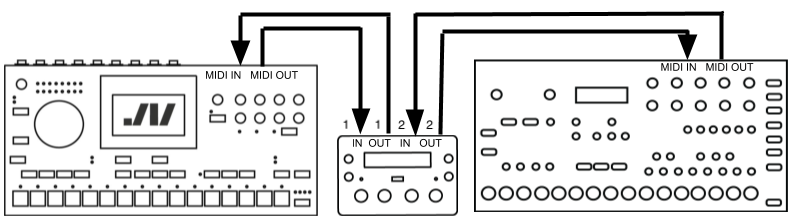
\includegraphics[scale=.6]{midi_machines.png}
\\
\newpage
\section{MachineDrum Settings }

MCL communicates with the MachineDrum using SYSEX messages, and will configure your MD's global settings automatically. MCL will overwrite and use MD's global settings slot 8. This slot should always be reserved for MCL.

\section{Analog4 Settings:}

The following configuration must be manually applied in the Analog 4's Global Settings menu:

\begin{itemize}

\item{MIDI Port Config:}
\begin{enumerate}
\item{Output to MIDI}
\item{Input to MIDI}
\item{Keyboard CFG = EXT}
\item{Receive Notes = True}
\item{Receive CC/NPRN = True}
\end{enumerate}
\item{MIDI Channels:}

Tracks 1-6 channels need to be set to MIDI Channels 1-6 respectively.

\end{itemize}

\section{Turbo MIDI}

MCL supports Elektron's Turbo MIDI protocol with selectable speeds 1x, 2x, 4x, 8x.\\
\\
Each MIDI port can be configured with a unique speed and is configurable in the \textbf{MIDI Menu} accessible from \textbf{Global Settings}.
\\
\\
\textit{For optimal firmware performance, reduced transmission latency and lowest sequencer jitter, use the default \textbf{Turbo 8x speed.}}

\section{Active Peering:}

When a MIDI device is connected to ports 1 or 2. The MegaCommand will automatically detect the attached device and set the chosen Turbo MIDI speed. If the attached device cannot be identified it will default to General MIDI (GM) Device. See \textbf{DEVICE 2} setting, in MIDI Settings Menu to specify the port 2 driver type.\\
\\
\textit{MCL has no fullproof method of detecting a snapshot change on the MachineDrum. If a new snapshot is loaded on the MD either the MC or MD will need to be power-cycled to reform the peer.}


 

\chapter{GUI}

\begin{center}
  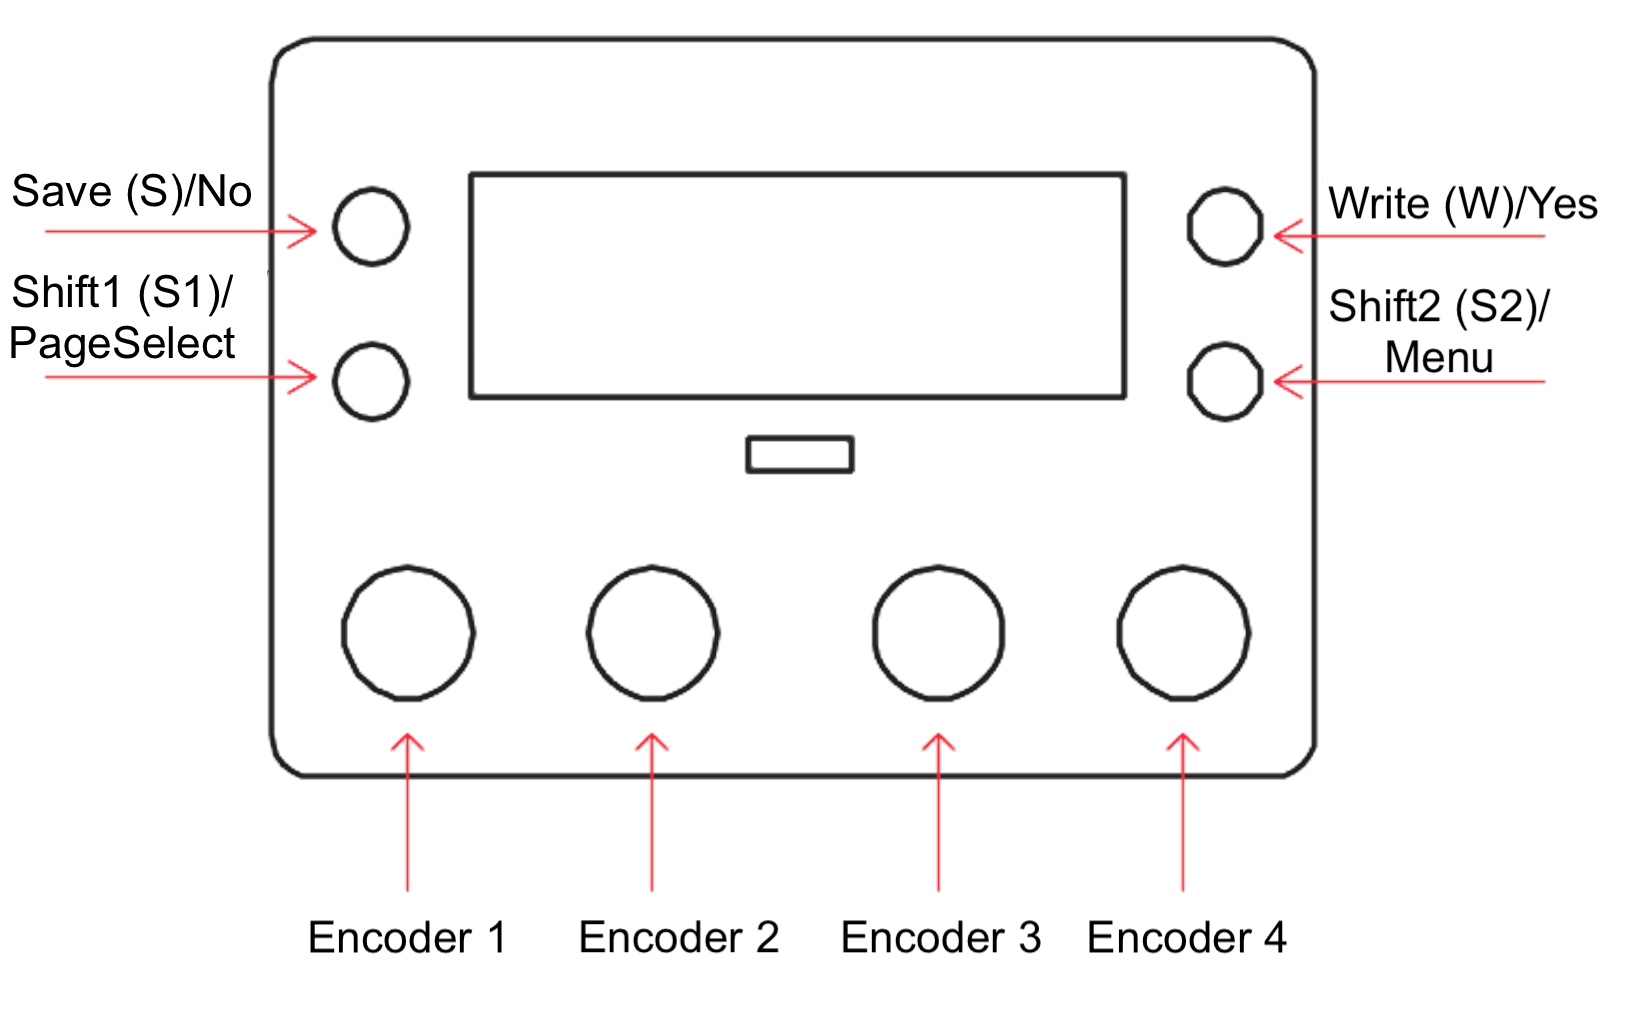
\includegraphics[width=16cm]{MC_Legend.png}
\end{center}

The MegaCommand's four upper function buttons are used to enter sub-menus and activate commands:
\section{Function Buttons:}
From the Grid Page the function buttons perform the following actions:
\begin{itemize}
\item{\textbf{[Save | No]}: Enters the Save Page}
\item{\textbf{[Write | Yes]}: Enters the Chain page}
\item{\textbf{[Shift1 | PageSelect]}: Enters the PageSelect page}
\item{\textbf{[Shift2 | Menu]}: Opens the slot Menu }
\end{itemize}
Combined Button Presses:
\begin{itemize}
\item{\textbf{[Save | No] + [Write | Yes]}: Opens the Global Settings menu }
\end{itemize}

\section{Encoder Buttons}
Encoder buttons are used to increase the speed of parameter rotation.
Holding down an encoder button whilst rotating the encoder will increase the update speed by 4x.

\section{Trigger Interface}
When connected to the Elektron MachineDrum, MCL will use the Machinedrum's 16 trigger buttons as additional GUI input. \\
\\
If connected to the Elektron AnalogFour (A4), MCL will use the A4's mini keyboard buttons as additional GUI input. Notes C,D,E,F are used to select A4 tracks 1,2,3,4 respectively.\\
\\
The Trigger Interface (TI) has different uses depending on the current page.\\
\\For example, the TI can be used to enter sequencer data in to the internal sequencer;
to select multiple tracks on the Mixer page and attenuate their volume simultaneously; to save or load Grid Slots from the Save or Chain pages and much more.

\subsection{Machinedrum OS Version}
As of MCL version 2.60, your machinedrum must be upgraded to OS version 1.70 or greater.


\chapter{Trigger Interface}
When connected to the Elektron MachineDrum, MCL will use the Machinedrum's 16 trigger buttons as additional GUI input. \\
\\
When connected to the Elektron Analog 4, MCL will use the A4's mini keyboard buttons as additional GUI input. Buttons C,D,E,F are used to select tracks 1,2,3,4 respectively.\\
\\
Depending upon the current page, the Trigger Interface (TI) works in a variety of ways.\\
\\For example, the TI can be used to enter sequencer data in to the internal sequencer;
to select multiple tracks on the Mixer page and attenuate their volume simultaneously; to save or load Grid Slots from the Save or Chain pages and much more.

\section{Trigger Interface Limitations}
The MD TI is not natively supported by the MD and is instead achieved using a Global Slot/MIDI Channel exploit. The exploit is used to differentiate between notes triggered by the sequencer and notes triggered by a user key-press.\\
\\
The TI will cease working whenever the MD display is updated unexpectedly, for example, when a machine parameter's value is changed; or when a sub-menu on the MD is opened.\\
\\
As a precaution, whenever entering a Page on the MC that uses the TI, the MD's current track will automatically change to a track without Parameter locks. This avoids unexpected display updates that may be caused by transmitted Parameter Changes. If all tracks have parameter locks, then Track 16 will be chosen. Parameter Locks on Track 16 will therefor not be transmitted when the TI is active.\\
\\
\textit{Recovery: If the Trigger Interface stops working exit all submenus on both the MD and MC. On the MD press \textbf{[ Func + Extended ]} to reset the state of the MD.}

\chapter{Page Select}
The PageSelect page is accessed by holding the \textbf{[Shift1 | PageSelect ]} button.
\\
\\
\fbox{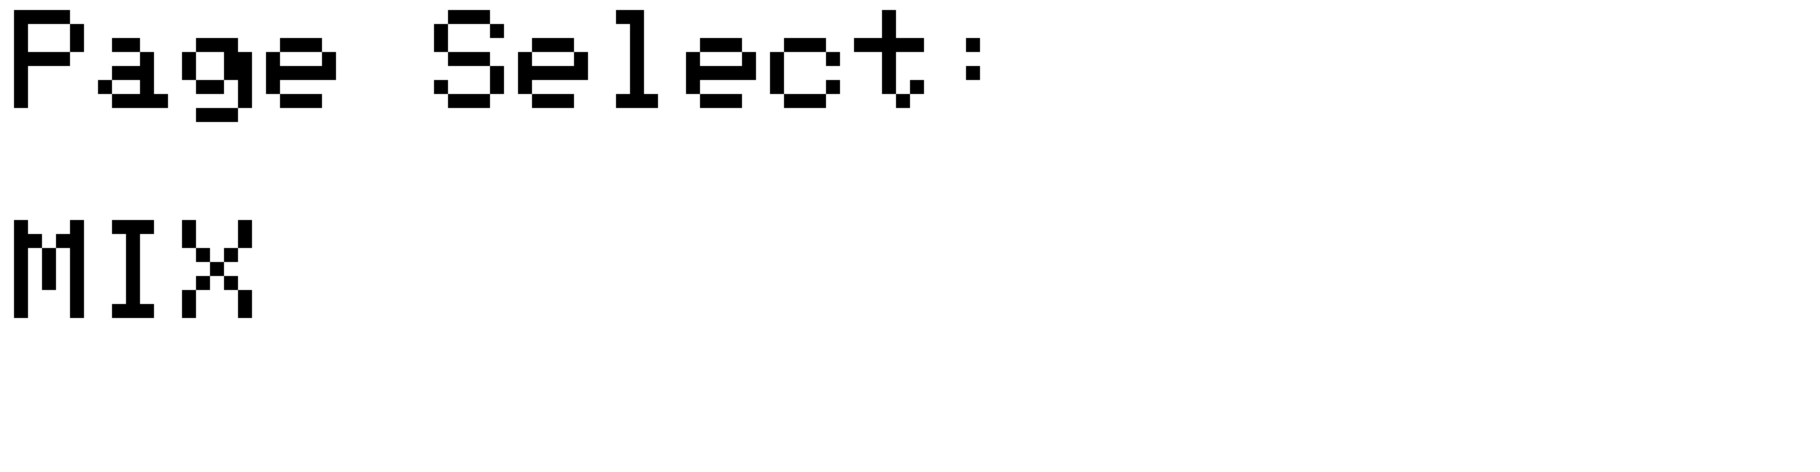
\includegraphics[scale=.4]{page_select_page.png}}\\
The PageSelect page allows quick access to auxillary pages not accessible through the main GUI buttons.\\
\\
When open, the PageSelect page displays the Page to be loaded, releasing \textbf{[Shift1 | PageSelect]} will load
the selected page.
\\
\\Rotating \textbf{[Encoder 1]} will scroll through the available PageSelect pages.
\begin{itemize}
	\item{1. Mixer Page}
	\item{2. Route Page}
	\item{4, RAM Page}
	\item{6, SoundBrowser Page}
	\item{7, Loudness Page}
    \item{8, Wav Designer}
\end{itemize}
\\
\textit{The MD's trigger interface can be used to quickly toggle between pages in the PageSelect page. }







\chapter{Global Settings Menu}
The Global Settings Menu is used for project management and to change a variety of software and hardware settings.

\screenshot{global_menu_1.png}
%\fbox{
\includegraphics[scale=.40]{global_menu_1.png}}\\\\
%\fbox{
\includegraphics[scale=.40]{global_menu_2.png}}\\

\textit{To enter the Global Settings menu press \textbf{[ Save ] + [ Write ]} from the GridPage.\\
To enter sub-menus press one of the Encoder Buttons. Use the function buttons to go back one level or exit the menu.}
\section{Load Project:}
The Load Project sub-menu will display a list of MCL Projects that are stored on the root folder of the Micro SD card.\\\\
The current project is always selected first and is indicated by an '>' character next to its name.
\screenshot{project_menu.png}
%\fbox{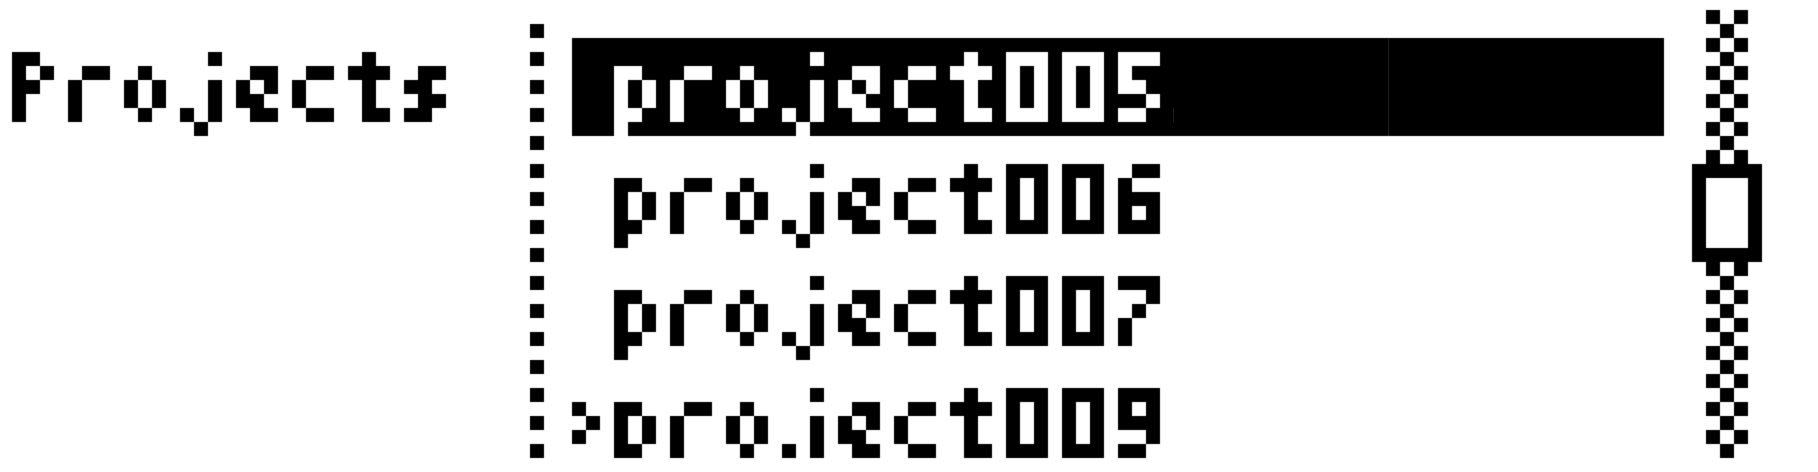
\includegraphics[scale=.40]{project_menu.png}}\\
\newpage
\section{New Project:}
The New Project options loads the New Project Page. This page allows you to specify a name for a project which will then be created.\\
%\fbox{
\includegraphics[scale=.40]{new_project.png}}\\
\screenshot{new_project.png}

\screenshot{charpane.png}
\textit{All text editing pages in MCL allow access to char pane. Hold \textbf{[Shift2]}}

\chapter{MIDI Settings Menu:}
The MIDI menu allows you to configure MIDI ports one and two.
\screenshot{midi_menu.png}
\\
\textit{Changes to MIDI settings are applied upon exiting the MIDI menu.}

%\fbox{
\includegraphics[scale=.40]{midi_menu.png}}
\section{Turbo MIDI:}
The TURBO MIDI speed can be set for each port (8x turbo is recommended for best performance.) To disabled turbo MIDI set the speed to 1x.
\section{MIDI Clock:}
MCL does not generate its own MIDI Clock, instead it relies on a clock signal from either port 1 or port 2.\\\\
The CLK REC parameter can be used to set the receive port for the MIDI clock.\\
The CLK SEND parameter can be used to forward the MIDI Clock from port 1 to port 2.\\\\
\textit{Note: The MD's clock settings are controlled by MCL and will be automatically configured based on the options selected above.}

\section{MIDI Forward:}
The MIDI FWD option allows you to forward non-realtime MIDI messages received on port 1 to the MIDI out of port 2 or vice versa.
\section{DEVICE 2: }
Set to either: General MIDI (Gener) or Elektron (Elekt)\\

This option sets the default MIDI driver for port 2. Supported Elektron devices have
more advanced features such as retaining kit/sound data when saving/loading slots,
The general MIDI driver will only save/load MIDI sequencer data.\\
\\
If you are intending to pair your Megacommand with an Elektron device
(MNM, A4) set this to Elektron. For all other MIDI devices, set this to General MIDI (new default setting).
\chapter{Machinedrum Settings:}
The Machinedrum settings are used to control how the MCL firmware interacts with the MD.
\fbox{
\includegraphics[scale=.40]{machinedrum_menu.png}}\\
\section{Kit Save:}
Before entering a Page, MCL will attempt to download the MD's current kit. In order to get an up to date version of the kit, it must first instruct the MD to save the current kit. You can choose to disable this behaviour by turning AUTO SAVE to off. By disabling this, some pages may not work correctly.
\section{Normalize:}
When activated, all saved tracks have their LEV boosted to 127, and parameters controlling VOL (including parameter locks) are lowered
to compensate. LFOs with destination VOL are 
adjusted too.\\
\\
The resulting track loudness remains the same, but the Track LEV parameter is no longer set arbitrarily. LEV == 127 will always be the loudest volume for each track.
\section{CTRL CHAN:}
The CTRL CHAN setting is used to specify which note data the MD responds to when in Chromatic modes. \\\\The default value is INT (internal) and states that the MD will be controlled by the Trigger Interface (TI) in chromatic mode. \\
\\If set to a channel number, the MD will be controlled by the specified MIDI channel on port 2. If set to OMNI the MD will be controlled by any channel on port 2.
\section{Poly Config}
The POLY CONFIG option opens the Voice Select page and allows 2 or more voices of the MD to act as voices of a polyphonic synthesizer.

\chapter{Chain Mode Settings Menu:}
The CHAIN setting enables or disables Chain Mode.\\\textit{See the "Chain Mode" chapter for more details.}

\screenshot{chain_menu.png}

\textit{Chain Mode can be enabled by selecting one of 3 three options: Automatic, Manual and Random.}
\\
\section{Chain:}
\begin{itemize}
\item \textbf{Automatic:} If the number of loops is greater than 0, slots will automatically jump to the specified Row after N loops.
\item \textbf{Manual:} Automatic slot jumping is disabled, tracks can be chained manually using the quantization rules in the Chain Page.
\item \textbf{Random:} Slots will jump after a random number of iterations to a random row position bounded by the min and max settings specified in Global Settings.
\end{itemize}
\section{Rand Min/Max:} The random min + max values are used to specify the minimum + maximum range of rows that will be loaded when random mode is enabled.

\chapter{System Settings Menu:}

\section{Display:}
The display setting is used to enable the OLED display mirror. Using the provided python script and a USB connection between the MC and your computer, it is possible to mirror the OLED display over the serial port to your computer screen.
\textit{Leaving this setting enabled will reduce the performance of the GUI.}
%\chapter{ Workflow: }

The Grid is similar to the banks of the MD, but different. An active pattern is first chain-written from the Grid into the Internal Sequencer and then ready for playback. 

Different tracks from different rows in the Grid can be mix-and-matched into the Internal Sequencer too.

Patterns created in the Sequencer Pages are kept in the Internal Sequencer, and thus not immediately saved to the Grid, until the MCL firmware is told so in the Save Page. 

A common gotcha is to create a pattern in the Sequencer Pages, use the Chain Write page to load data from the Grid, only to find the just-created pattern gone. To avoid this, make sure to \textbf{save modified internal sequence before chain write}.

\chapter{Grid Page}
The first page you will be presented with after loading or creating a new project is the Grid Page. This is the main page of MCL and is used to access the firmware's sub-pages and menus.

\begin{center}
	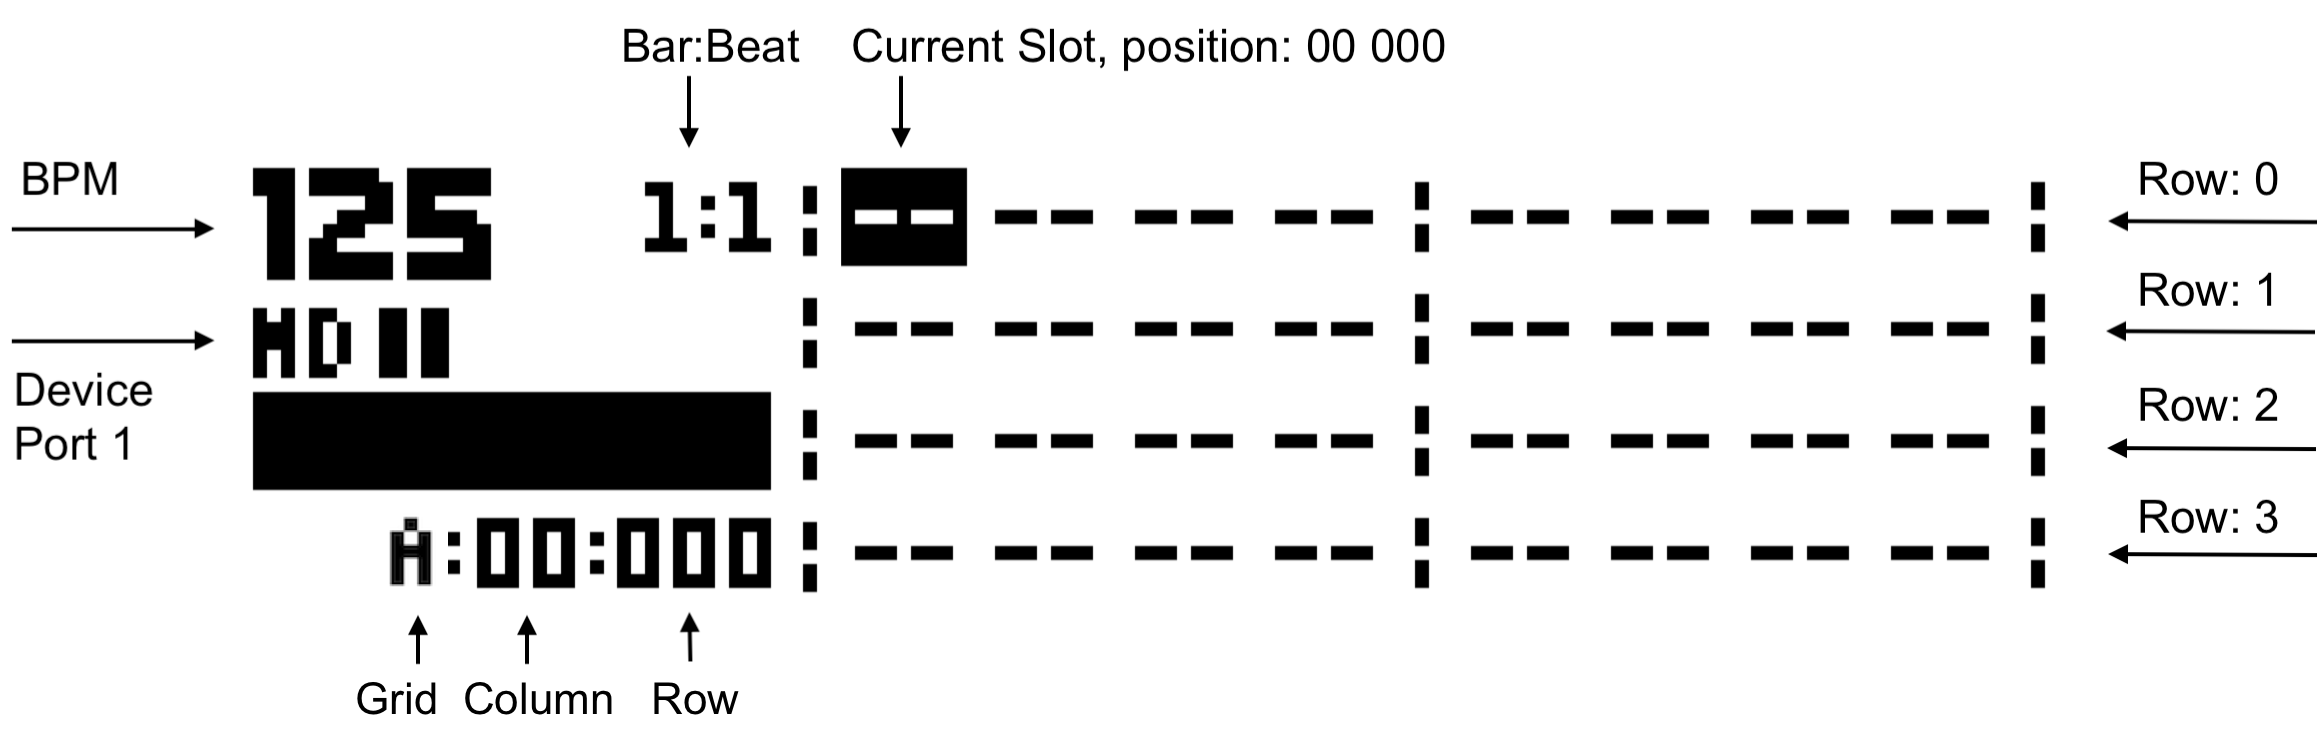
\includegraphics[scale=.40]{grid_init_annot.png}
\end{center}
MCL displays a portion of the active grid on screen. 
Eight slots across four rows are shown.\\
\\
Occupied slots will display the Machine Type associated with the track. For example "BD" for Bass Drum. Unoccupied Slots are represented by two lines of "--" . For clarity, a dashed vertical line is printed after every fourth column.\\\\
An interactive cursor indicates the current slot position and is distinguished by a slot printed with inverted colours. Rotating \textbf{[ Encoder 1 ]} or \textbf{[ Encoder 2 ]} will allow the cursor position to change. When the cursor reaches the edges of the screen you can continue to scroll through the grid.
\\\\
Towards the bottom left corner of the display, the active grid followed by the current slot's column and row are shown.\\\\
The active grid can be toggled between either A or B from the Slot Menu.
\textit{When performing actions such as saving/loading they will apply to the grid that is currently active.}
\\
\encodersbuttons{scrolls the grid horizontally.}{scrolls the grid vertically.}{--}{--}{activates Save page.}{activates PageSelect page.}{activates Load page.}{activates the Slot menu.}
\chapter{Grid/Slot System:}

%\begin{center}
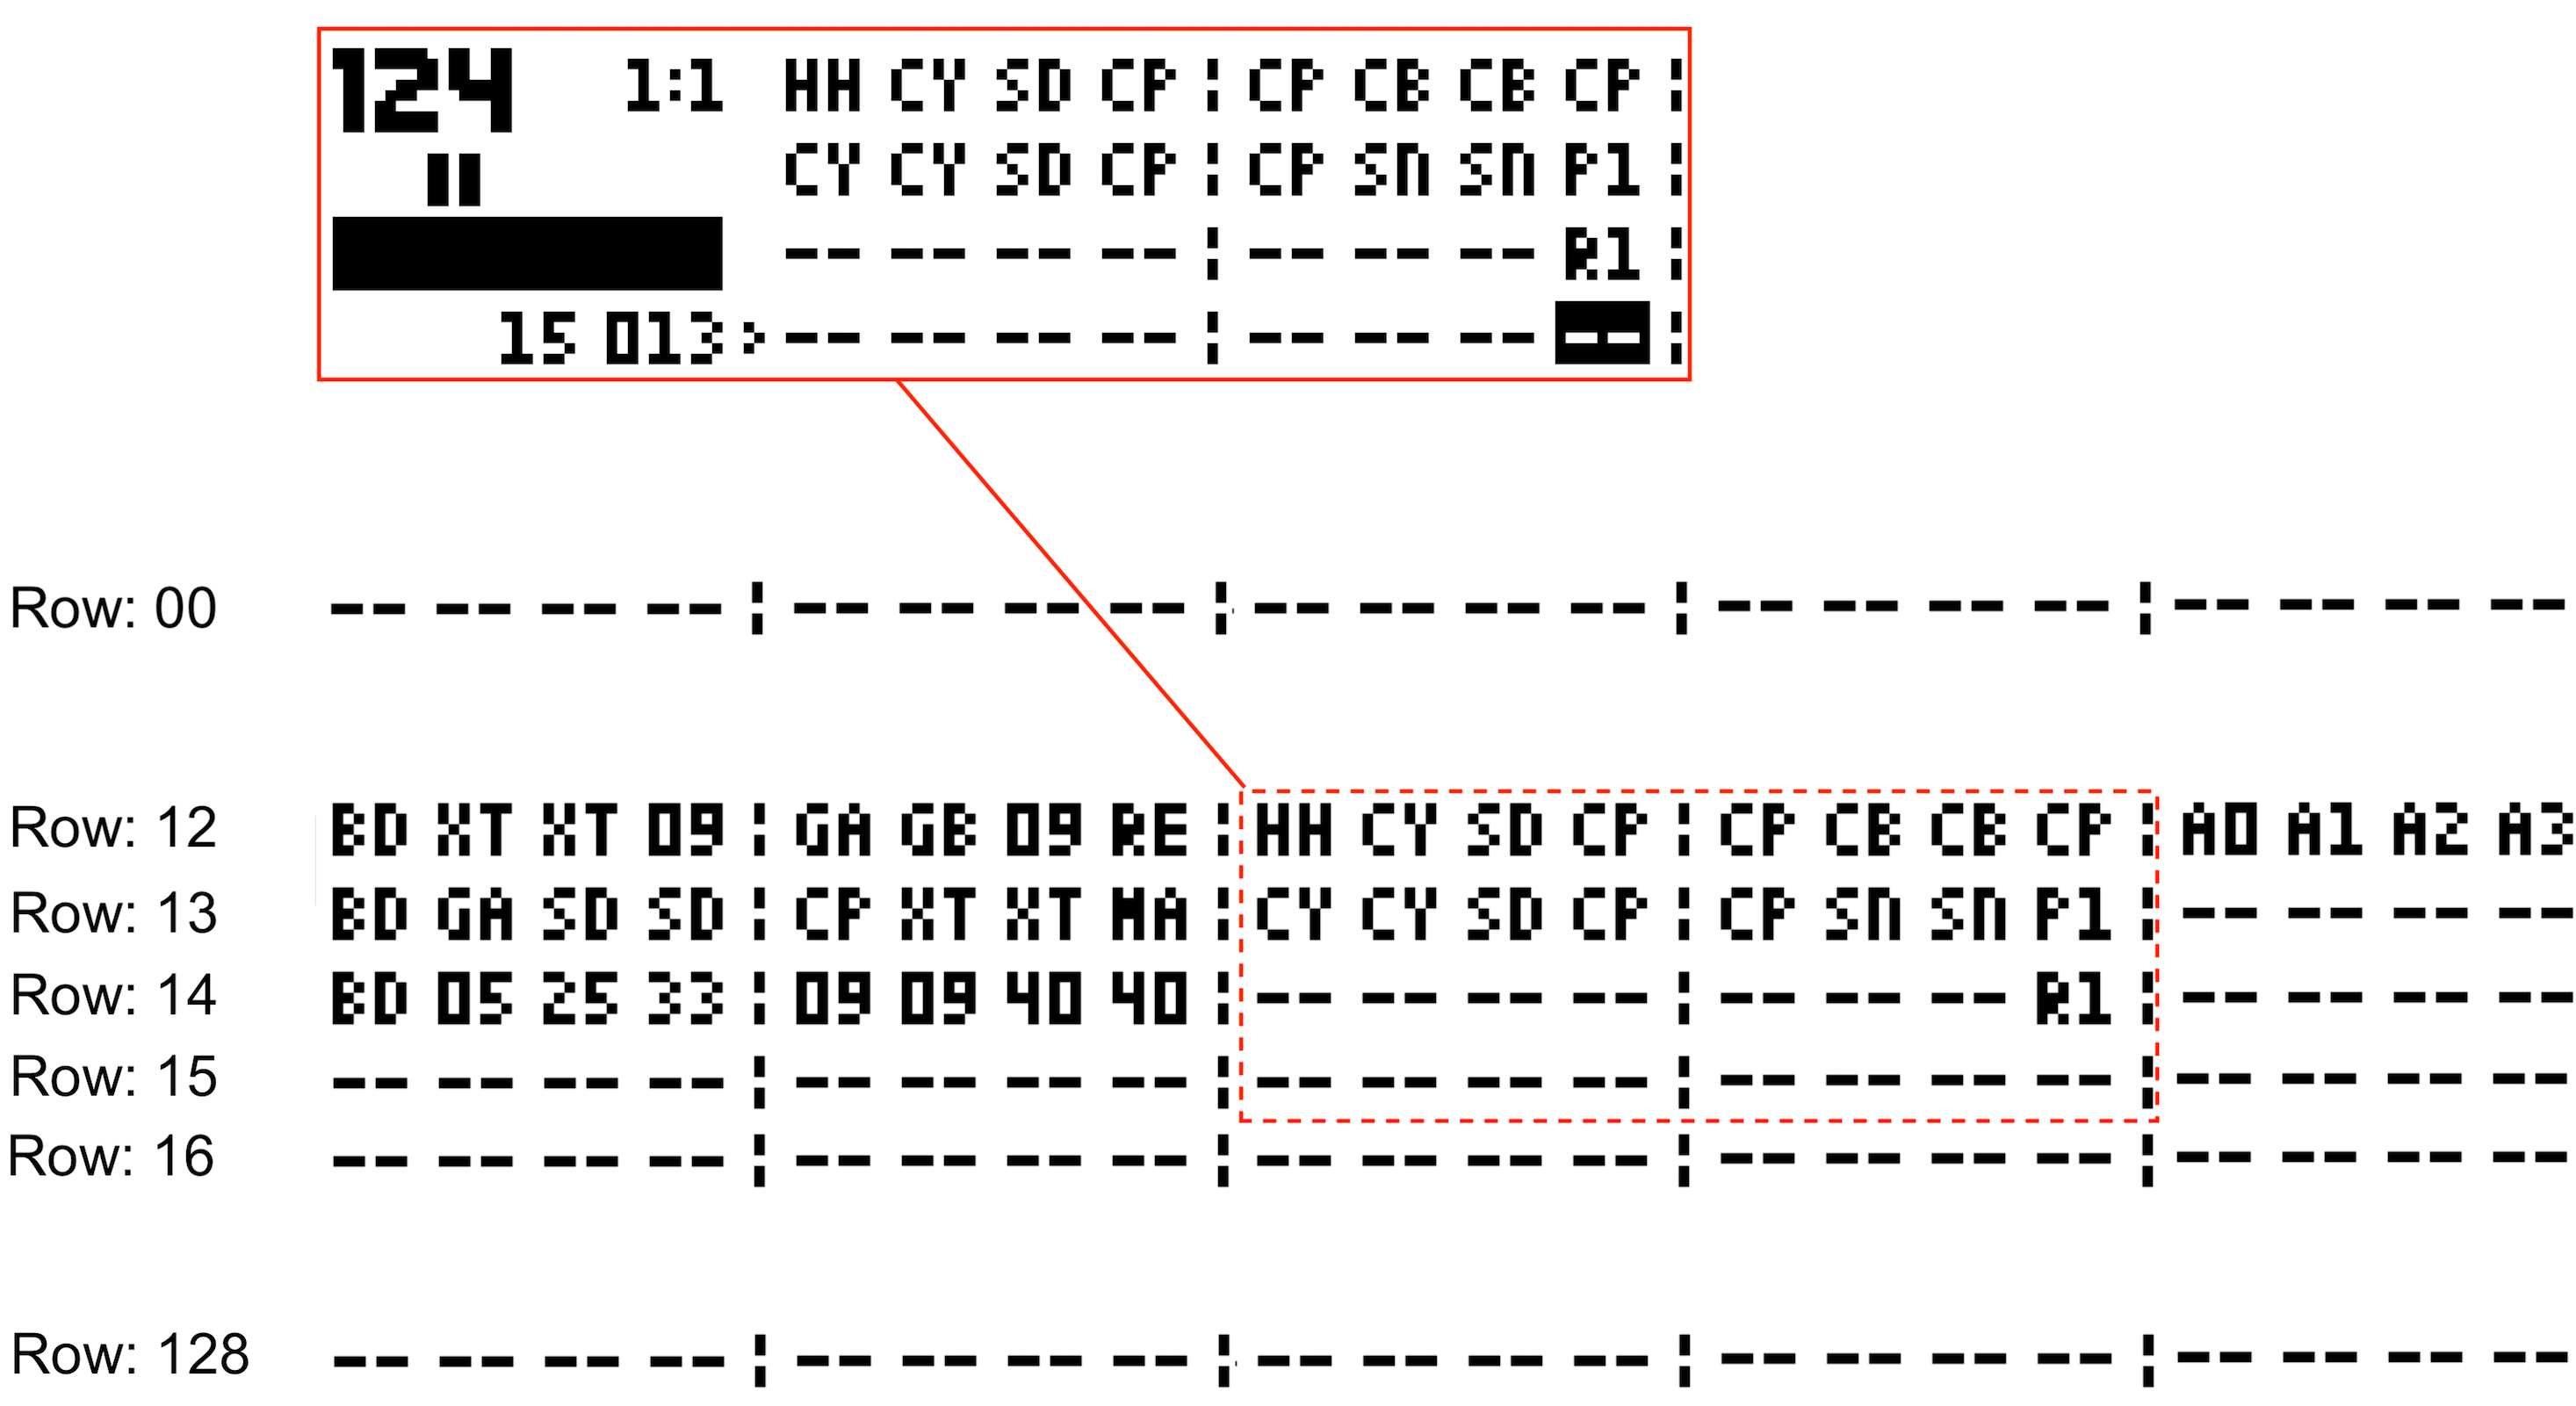
\includegraphics[scale=1.0]{grid_enlarged.png}
%\end{center}
\\\\
The Grid is a data structure consisting of 128 rows with each containing 20 slots. \\
\\
The first 16 slots of a row are reserved for MD tracks. The remaining 4 slots are used for Analog4 or External MIDI tracks.



\chapter{Slot Menu:}

The Slot Menu is an important sub-menu of the Grid Page and is used to manipulate slots in a variety of ways. It can be used to clear, copy, paste one or more slots in a row or to configure a slot's chain settings. It also provides an option to rename the current row and provides a quick way to activate or deactivate various Global Chain Modes.
\screenshot{slot_menu.png}
%\fbox{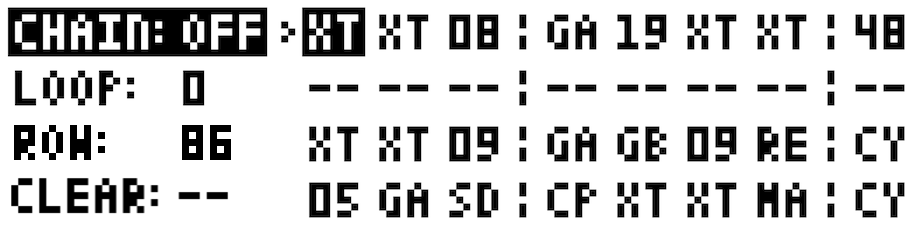
\includegraphics[scale=.40]{slot_menu.png}}\\
\\
\textit{The SlotMenu is accessible from the GridPage by holding down the  \textbf{[Shift2]} function button.\\
When \textbf{[Shift2]} is released, any changes to the menu will be applied to the selected slots. }
\\
\section{Multiple Slot Selection:}
A rectangular selection consisting of multiple slots can be made by rotating \textbf{[Encoder 1]} and \textbf{[Encoder 2]}.

\screenshot{range_copy.png}

\section{Slot Menu Options:}
Slot Menu has the following options and selectable values:

\begin{tabular}{|l|l|}
\hline
\rowcolor[HTML]{C0C0C0} 
Entry                                  & Function                                                                                                                                                                                      \\ \hline
Chain: {[} –, auto, manual, random {]} & \begin{tabular}[c]{@{}l@{}}auto: enables chain auto mode global setting.\\ manual: enables chain manual mode global setting.\\ random: enables chain random mode global setting.\end{tabular} \\ \hline
Loops: (0, 64)                         & specify how many times to loop track/slot.                                                                                                                                                    \\ \hline
Row: (0,127)                           & \begin{tabular}[c]{@{}l@{}}specify which row, the current slot is to\\ load/jump to after n loops.\end{tabular}                                                                               \\ \hline

Clear: {[} –, YES {]}                  & clear the selected slot(s).                                                                                                                                                                   \\ \hline
Copy: {[} –, YES {]}                   & copy the selected slot(s).                                                                                                                                                                    \\ \hline
Paste: {[} –, YES {]}                  & paste the selected slot(s).                                                                                                                                                                   \\ \hline
Rename                                 & rename the current row.                                                                                                                                                                       \\ \hline
\end{tabular}

\section{HD44780 LCD users:}
\textit{Note: For users running MCL on a \textbf{HD44780 LCD}, the SlorMenu  is accessible from the GridPage by holding down the  \textbf{[Shift2]} function button and pressing a corresponding encoder button.\\
\\For example if slots 5 to 8 are displayed on screen, holding  \textbf{[Shift2]} and then pressing \textbf{[Encoder3]} will open the slot menu for slot 7.}\\
\\
Rectangular selection is not available for the HD44780. Instead, an additional "APPLY" parameter is provided. If the APPLY value is greater than 1, changes will be applied sequentially; starting from the current slot and up to the number of slots specified by the APPLY value on the same row.


\chapter{Internal Sequencer:}
MCL features a powerful 20 track internal sequencer. There are 16 tracks dedicated to the MD and 4 tracks dedicated to the Analog 4 or an External Midi device.
\section{MD Sequencer Tracks:}
\begin{itemize}
\item 16 Track Sequencer with independent track lengths (64 max steps).
\item Conditional Trigs and Micro Timing per step (10 degrees left or right of centre.)
\item 4 lockable parameters per track with 64 locks per parameter. Lockable parameters are MIDI learnt and recordable from the MD.
\item Trigless Locks.
\item Real time record for both step and lock data.
Chromatic Mode. (Machine pitch values are chromatically mapped to the MD. Melodies are recordable)
\end{itemize}
\section{A4 or ExtMIDI Sequencer tracks:}
\begin{itemize}
\item 4 x 4-Note Polyphonic On-Off sequencer tracks. Each track can run in either high or low resolution modes. 
\item Each track transmits on MIDI-OUT2, Midi channel = Track Numbers 1 to 6.
\item Conditional Trigs and MicroTiming (6 degrees for high res, 10 degrees for low res)
\item Low resolution mode up to 128 steps per track,
\item High resolution mode up to 64 steps per track with the ability trigger successive 16th notes.
\item Chromatics Mode with selectable scales.
\item Legato record
\end{itemize}
The internal sequencer is synced to the MIDIClock source.
\\
\section{Internal Sequencer: Loading and Saving}
Internal sequencer tracks are linked to the slot positions in the Grid.\\
\\
When storing a track within the Save menu, the internal sequencer data for that track is stored along with the track data in the specified slot.\\
\\
Internal Sequencer tracks are loaded when tracks are sent to the MD or A4 in the Write page.

\section{Internal Sequencer Pages:}
\textit{The primary Sequencer Pages are accessed using [\textbf{Encoder Buttons (1-4)].} Each sequencer page has access to secondary pages accessible by pressing \textbf{[Save]}}

\begin{itemize}
	\item Encoder 1: MD Step edit                          [ A4 Step edit ]
	\item Encoder 2: MD Record Live                      [ MD Record Parameter Locks Live ]
	\item Encoder 3: MD Parameter Lock Page A  [ MD Parameter Lock Page B ]
	\item Encoder 4: MD/A4 Pitch Mode                [ MD/A4 Pitch Record Mode ]
\end{itemize}
\chapter{Save Page}

The Save Page is used to copy track data from the Machinedrum to a specific slots in the current row of the Grid. \\
\\
When a track is saved to a slot, the MC's internal sequencer data for that track is also stored alongside the copied track data.\\
\\
Master Effects settings are also saved with each MD Track.
\\\\
\textit{The Save Page is accessible from the GridPage by pressing the  \textbf{[Save]} function button.}
\\\\
	\fbox{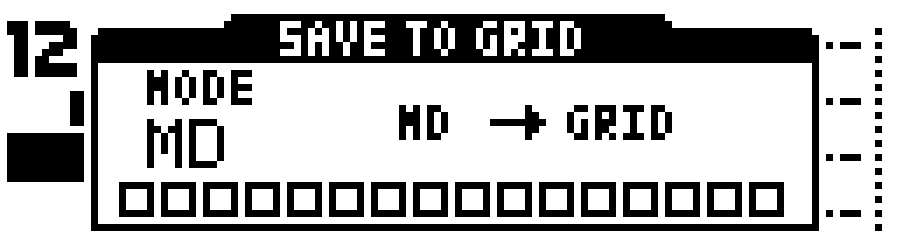
\includegraphics[scale=.40]{save_page.png}}
\section{Encoder Assignment:}
\begin{itemize}
	\item \textbf{[ Encoder 1 ]: }Source Bank
	\item \textbf{[ Encoder 2 ]: }Source Pattern
	\item \textbf{[ Encoder 3 ]: }--
	\item \textbf{[ Encoder 4 ]: }--
\end{itemize}
\section{Saving Tracks}
The Save Page uses the Trigger Interface to specify which tracks are to be saved. Pressing multiple triggers on the MD and then releasing them will cause the selected tracks to be stored in the corresponding slots of the current row.\\
\\
The default behaviour is to store tracks to slots in a one-to-one mapping. That is to stay. Pressing triggers 1,2,3,4 will store MD tracks 1,2,3,4 in MC slots 1,2,3,4 of the current row.\\
\\
Holding  \textbf{[Shift1]} will cause the mapping to be offset by the MD's current track number. For example: If the MD currently has track 5 selected and triggers 1,2,3,4 are chosen then the MD Track's 5,6,7,8 will be stored in slots 1,2,3,4 of the current row.
\section{Store a pattern/row:}
To save an entire pattern/row press \textbf{[Shift2]} from within the Save Page.
All A4 sounds or external sequencer data will also be saved.



\section{Pattern Selection:}

Changing the Bank+Pattern allow you to specify the MD's source pattern location. The MD’s currently loaded pattern and kit are used by default

\chapter{Chain Mode:}
Chain mode was inspired by old school music tracker software that generate music by iterating through sequences and sounds stored in in vertical columns.
\section{Functionality:}
Each slot in the Grid has the ability to play for N loops and then jump to another slot in a specific row of the same column.  These values are specified by the LOOPS and ROW settings in the SlotMenu and apply to the current slot. Jumping between slots is referred to as a transition. Just before a transition occurs, Machine settings are sent to the MD and the internal sequencer data for that track is loaded. All 20 tracks can be configured to transition at the same time.\\
 \\
Chain mode will not send pattern data to the MD. Therefor you must perform all your sequencing using MCL's internal sequencer. For your convenience it is possible to merge a slot's MD sequencer data from within the Save Page.
\section{Modes of Operation}
\textit{Chain Mode behaviour can be changed in the SlotMenu or GlobalSettings-->ChainMode menu by setting ChainMode to one of 3 three settings: Automatic, Manual and Random.}

\begin{itemize}
	\item Automatic: If the number of loops is greater than 0, slots will automatically jump to the specified Row after N loops.
	\item Manual: Automatic slot jumping is disabled, but tracks can be chained using the quantization rules in the Chain Page.
	\item Random: Slots will jump after a random number of iterations to a random row position bounded by the min and max settings specified in GlobalSettings-->Chain Mode
\end{itemize}



\chapter{Chain Page}
When chain mode is enabled the Write Page is replaced with the Chain Page.\\
\\
The chain page allows you to manually load slots at a specific transition interval defined by the Quantization rules.\\
\\
The minimum Quanitization value is 4 steps. Quantization values can be changed by adjusting the "Q:" parameter.
\\\\
\textit{When Chain Mode is enabled, the Chain Page is assessable from the GridPage by pressing the  \textbf{[Write | Chain]} function button.}
\\\\
\fbox{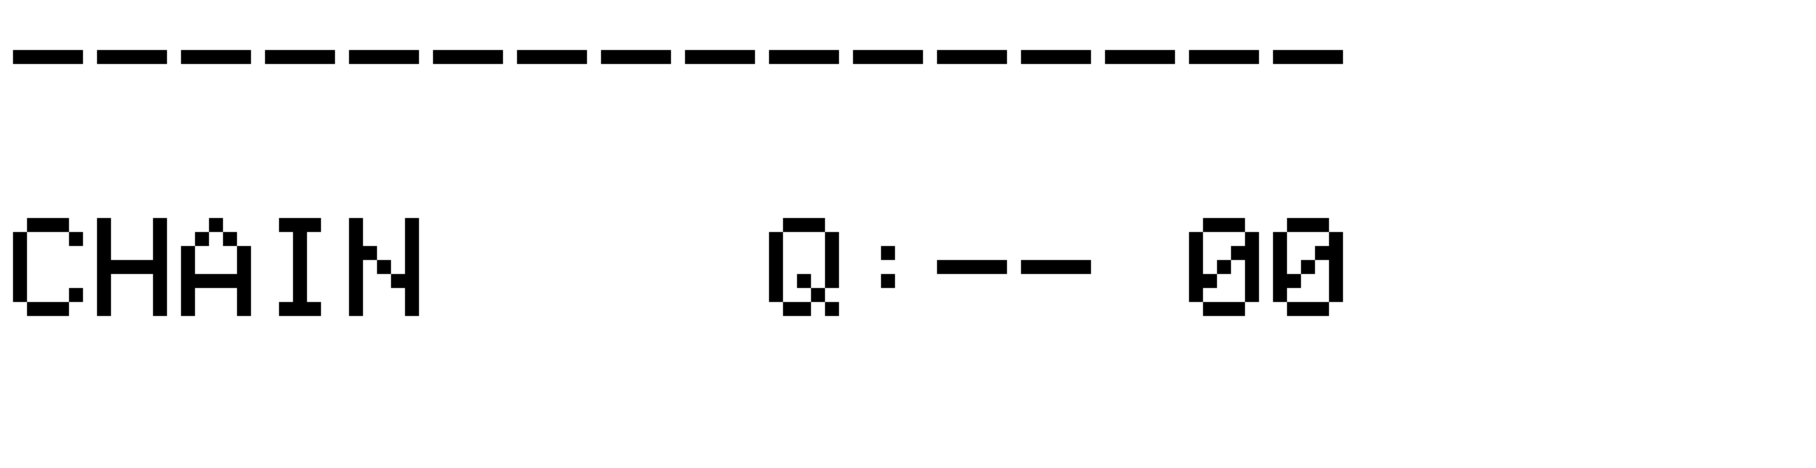
\includegraphics[scale=.40]{chain_page.png}}\\
\section{Encoder Assignment:}

\begin{itemize}
	\item \textbf{[ Encoder 1 ]: } --
	\item \textbf{[ Encoder 2 ]: } --
	\item \textbf{[ Encoder 3 ]: } Quantization (Q)
	\item \textbf{[ Encoder 4 ]: }--
\end{itemize}

\chapter{Internal Sequencer Pages:}

\textit{The primary Sequencer Pages are accessed using the \textbf{PageSelect} page. Each sequencer page has access to secondary pages accessible by pressing \textbf{[Save]}}
\begin{itemize}
	\item MD Step edit                          [ A4 Step edit ]
	\item MD Record Live                      [ MD Record Parameter Locks Live ]
	\item MD Parameter Lock Page A  [ MD Parameter Lock Page B ]
	\item MD/A4 Pitch Mode                [ MD/A4 Pitch Record Mode ]
\end{itemize}
\section{Track selection}
To change the current track in a sequencer page, simply change tracks on the MD. 
\\\\
\textit{Automatic track select can be disabled from the MCL system menu option Global -> Machinedrum -> TRACK SELECT}
\section{Track menu}

\vspace{-10pt}

\screenshot{track_menu.png}

The track menu will be opened when holding \textbf{[Shift 2]}, and the entry activated on release, similar to the slot menu.
The track menu consists of the following entries:

\begin{figure}[hb]
    \begin{tabular}{|l|l|}
    \hline
    \rowcolor[HTML]{C0C0C0} 
    Entry            & Function                                                                                                                \\ \hline
    Track Select     & select active track                  *only visible when TRACK SELECT = MAN                                              \\ \hline
    Copy             & \begin{tabular}[c]{@{}l@{}}TRK: copy track\\ ALL: copy pattern\end{tabular}                                             \\ \hline
    Clear            & \begin{tabular}[c]{@{}l@{}}TRK: clear track\\ ALL: clear pattern\end{tabular}                                           \\ \hline
    Paste            & \begin{tabular}[c]{@{}l@{}}TRK: paste track\\ ALL: paste pattern\end{tabular}                                           \\ \hline
    Track Resolution & \begin{tabular}[c]{@{}l@{}}toggle between hi/low resolution\\ on external tracks.\end{tabular}                          \\ \hline
    Shift            & \begin{tabular}[c]{@{}l@{}}L/R: shifts the track left/right.\\ L ALL/R ALL: shifts the pattern left/right.\end{tabular} \\ \hline
    Reverse          & TRK: reverse the trackALL: reverse the pattern                                                                          \\ \hline
    \end{tabular}
\end{figure}
\chapter{MD StepEdit Page:}

The MD StepEdit page is used to program MCL's internal sequencer for a selected track. The programmed sequence will run alongside the MD's sequence for the same track.

\screenshot{step.png}

\textit{To enter the MD StepEdit Page: First select desired track on the MD \textbf{[Function + Track N]}. Then press \textbf{[PageSelect + Trigger 5]}.}

%\fbox{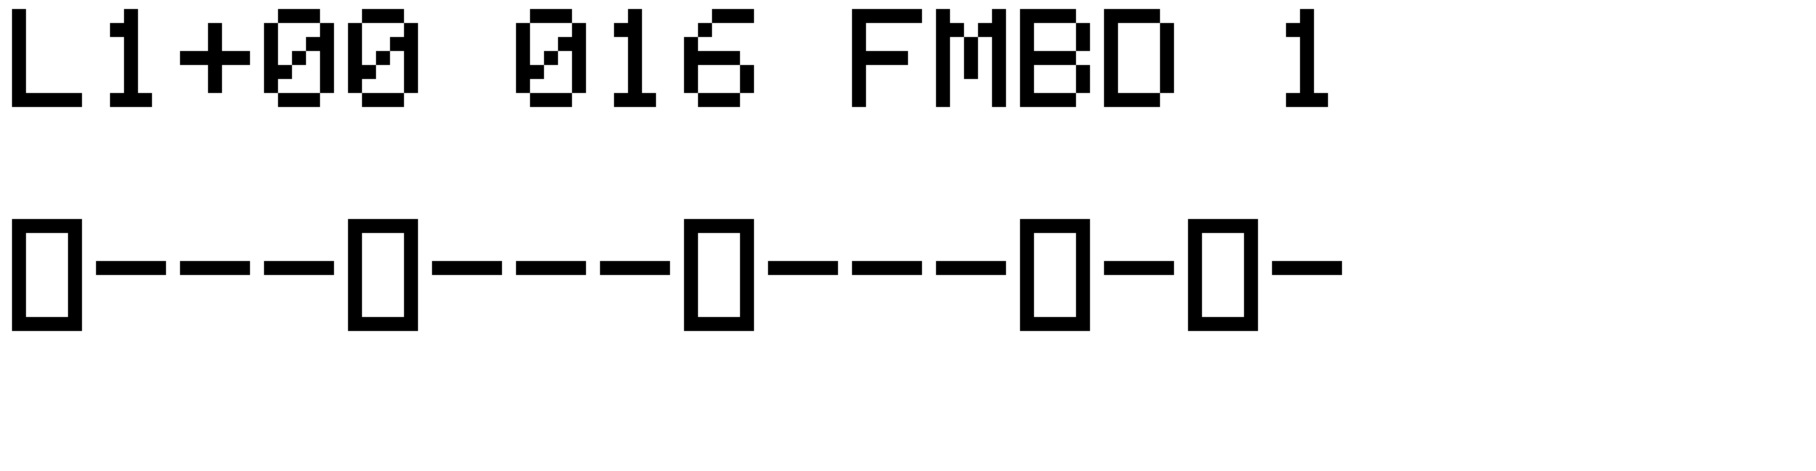
\includegraphics[scale=.40]{seq_step_page.png}}
\screenshot{step_action.png}

\encodersbuttons{Trig Condition}{Micro-Timing}{Track Length}{Note}{Toggles MD/Ext}{PageSelect}{Rotate View}{Track/Trig Menu}

\section{GUI:}
\begin{itemize}
\item The Step Edit Page uses the TI. The trigger buttons on the MD correspond to the 16 steps on the current page of the current track.
\item The 16 steps are displayed on the bottom row
\item Trig Conditions and Micro-Timing settings are per step and are chosen from encoders 1 and 2 respectively.
\end{itemize}

\section{Trig Conditions:}
\begin{itemize}
\item L1,L2,L3,L4,L5,L6,L7,L8 (For Ln, step is only triggered after every n iterations of track)
\item P10, P25, P50, P75, P90 (For Pxx, step has a xx percent chance of being triggered)
\item 1S. (One Shot trig, step is only triggered once)
\end{itemize}
\section{Micro Timing:}
\screenshot{utiming1.png}

\vspace{-0.3cm}

\section{Program a sequence:}
\begin{itemize}
\item Press and hold trigger button(s) on the MD to place triggers in the sequence.
\item Rotate encoders 1 and 2 to change the conditional mode or micro-timing if desired.
\end{itemize}

\vspace{-0.3cm}

\section{Clearing a sequence:}
\begin{itemize}
\item To clear the current track, press and hold the\textbf{ [ Shift2 ]} to open the track menu, rotate \textbf{[Encoder2]} to the entry \textbf{CLEAR}, then rotate \textbf{[Encoder1]} to select \textbf{TRK}.
\item To clear all MD tracks, select \textbf{ALL}
\end{itemize}

\vspace{-0.3cm}

\section{Rotating visible sequence:}
Each track consists of 4 pages of 16 steps, for a total of 64 steps per track.
\begin{itemize}
\item Rotate the current track-page by pressing the \textbf{[Write] }button.
\end{itemize}

\vspace{-0.3cm}

\section{Changing track length:}
\begin{itemize}
\item Track length is controlled by rotating \textbf{[ Encoder 3 ]}. Only steps less than the current track length are drawn.
\item To change the lengths of all 16 tracks simultaneously hold down \textbf{[Write]} whilst rotating \textbf{[ Encoder 3 ]}.
\item Track length can also be set by holding \textbf{[Write]} and then selecting the corresponding step from the MD trigger interface. The track length is offset by the current track-page.
\end{itemize}

\section{Chromatic Step Edit:}
The step page allows you to adjust a step's pitch by setting a note value. 
\begin{itemize}
\item Press and hold trigger button(s) on the MD. Rotating \textbf{[ Encoder 4 ]} will allow you change the note value of the selected steps.
\item A keyboard will be drawn on the display, showing the current note.
\end{itemize}
\screenshot{step_keyboard.png}

\chapter{PianoRoll Page:}
The PianoRoll page is used to edit External MIDI sequencer tracks 1-6.\\
The editor features two modes: Note editing and Automation editing.
\screenshot{proll.png}
\\
\textit{Press \textbf{[ PageSelect ] + [ Trigger 5 ]} to open the Pianoroll Editor page}
\encodersbuttons{Cursor X}{Cursor Y / Note Value}{Cursor Width / Note Width }{Zoom}{Record}{PageSelect}{Add or Remove Note}{Pianoroll Menu}
\section{Using the PianoRoll Editor:}
\screenshot{proll_edit.png}
The PianoRoll works in continuous time. The finest resolution is 1/192th per quater note. The cursor can be moved to a specific time offset by rotating \textbf{[ Encoder 1]}. \textbf{[ Encoder 4 ]} adjusts the zoom along time the time axis. The note value is chosen using \textbf{[ Encoder 2 ]} and the note width controlled using \textbf{[ Encoder 3 ]}.\\
Notes can be both entered and deleted by pressing the \textbf{[ Load ]} button.\\
\newpage
The MD Trigger Interface can be used to position the cursor at screen intervals of 1/16th.\\
Note width can also be adjusted by holding one MD Trigger button and then pressing another.\\\\
An external MIDI keyboard connected on port 2 can also be used to change the note value.\\
Using a simultaneous combination of the MD Trigger Interface and an external MIDI Keyboard, chords can be entered into the Note Editor.
\section{Live Record:}
Live Record mode can be activated by pressing  \textbf{[ Save ]}. Both note and automation \\(ControlChange) data can be recorded. All 8 tracks can be recorded to simultaneously.
\\Tracks will only record incoming data that is on the same MIDI Channel. \textit{(see section MIDI Channel Selection)}

\section{PianoRoll Menu:}
\screenshot{proll_menu.png}
Holding \textbf{[ Shift 2 ]} opens the PianoRoll menu. For each track you can adjust the MIDI Channel, track length and playback speed. Cursor editing options are also included here including note velocity and note conditional settings.

\begin{figure}[hb]
    \begin{tabular}{|l|l|}
    \hline
    \rowcolor[HTML]{C0C0C0} 
    Entry        & Function \\ \hline
    Track Select & Change Track \\ \hline
    Edit         & Note or Automation modes\\ \hline
    VEL         & Note Velocity\\ \hline
    Cond        & Trig Condition\\ \hline
    Channel     & MIDI Channel\\ \hline
    \end{tabular}
\end{figure}
\section{Change Edit Mode:}
From the PianoRoll menu, the "Edit" parameter changes the editing mode. Switch between either Note editing, or editing automation parameters 1-8.

\newpage
\section{Automation Editing}
\screenshot{proll_aut.png}
\textit{The PianoRoll Editor page allows for automation editing. From the PianoRoll menu, use the "Edit" menu option to select one of eight Automation Parameters.}
\\\\
Each External MIDI track features 8 automation parameters.
\begin{figure}[hb]
    \begin{tabular}{|l|l|}
    \hline
    \rowcolor[HTML]{C0C0C0}
    Entry        & Function \\ \hline
    Track Select & Change Track \\ \hline
    Slide      & Linear slide between automation values \\ \hline
    CC         & CC destination, Program Change,  MIDI learn \\ \hline
    \end{tabular}
\end{figure}
\\
Slide: enables/disable interpolation between automation events.\\\\
CC: allows a specific MIDI Control Channel number to be chosen.per parameter, Alternatively you can select LEARN, to Automatically learn the next received CC. When set to PRG, the track will send Program Change messages.

\section{MIDI Channel Selection}
Each Ext MIDI track listens and transmits on a set MIDI Channel. The channel defaults to the track number. This can be easily changed by modifying the PianoRoll menu CHAN option.\\

\chapter{MD Realtime Record Page:}

The RTRK Page is used to record tracks in real-time. If the sequencer is running, trigger presses on the MD will be recorded.

Thanks to micro-timing, trigger presses are recorded at 1/192th note resolution and have a much more organic feel than the MD’s real-time record mode.

\textit{To enter RTRK Page: First select desired track on the MD \textbf{[Function + Track N]}. Then press \textbf{[PageSelect + Trigger 6]}.}

%\fbox{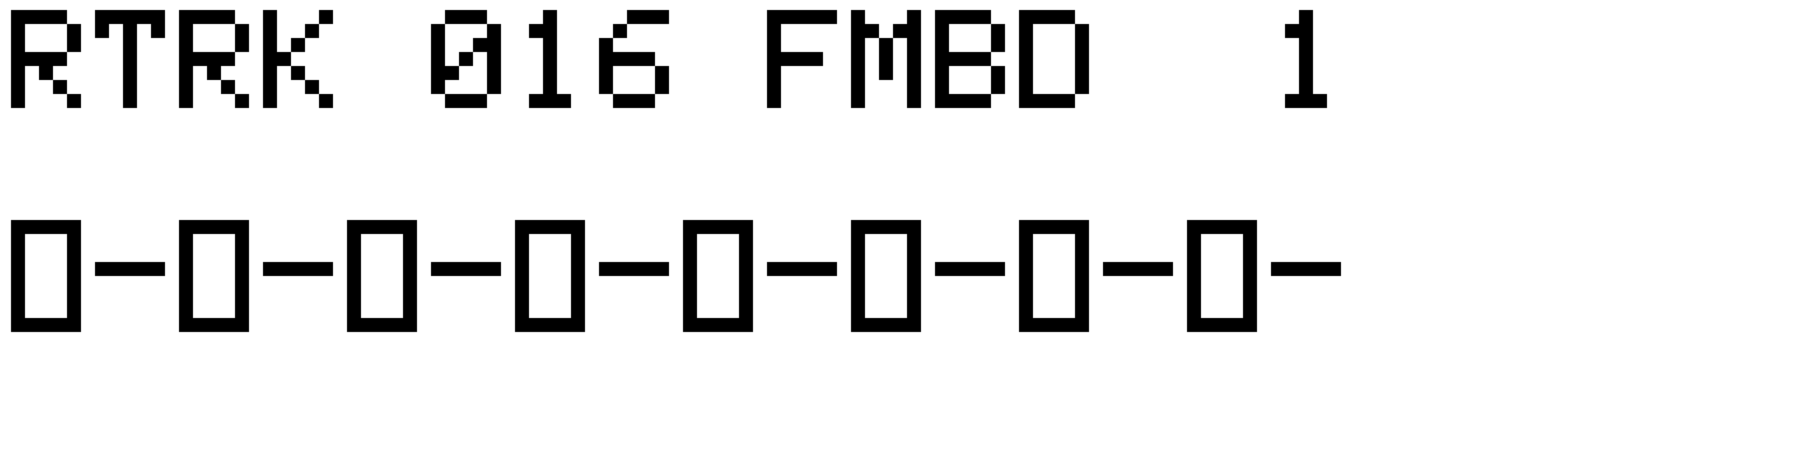
\includegraphics[scale=.40]{rtrk_page.png}}
\screenshot{rtrk_action.png}

When in RTRK Page, the current sequencer Track will automatically change according to the track corresponding to the last MD Trigger pressed.\\
\\To minimise record latency the display is prevented from updating unless a GUI action occurs. 

\encoders{--}{--}{Track Length}{--}

\section{Clearing a sequence:}
\begin{itemize}
\item To clear the current track, press and hold the\textbf{ [ Shift2 ]} to open the track menu, rotate \textbf{[Encoder2]} to the entry \textbf{CLEAR}, then rotate \textbf{[Encoder1]} to select \textbf{TRK}.
\item To clear all MD tracks, select \textbf{ALL}
\end{itemize}

\vspace{-0.3cm}

\section{Rotating visible sequence:}
Each track consists of 4 pages of 16 steps, for a total of 64 steps per track.
\begin{itemize}
\item Rotate the current track-page by pressing the \textbf{[Write] }button.
\end{itemize}

\vspace{-0.3cm}

\section{Changing track length:}
\begin{itemize}
\item Track length is controlled by rotating \textbf{[ Encoder 3 ]}. Only steps less than the current track length are drawn.
\item To change the lengths of all 16 tracks simultaneously hold down \textbf{[Write]} whilst rotating \textbf{[ Encoder 3 ]}.
\item Track length can also be set by holding \textbf{[Write]} and then selecting the corresponding step from the MD trigger interface. The track length is offset by the current track-page.
\end{itemize}


\chapter{Parameter Locks:}
The internal sequencer implements parameter locks for the 16 MD tracks. Each of these track has access to 4 Parameter Locks, with 64 steps per lock. Trigless locks are supported, meaning parameter values can change without retriggering the sound. \\\\Unique characters are used to represent the types of locks and are discussed below.
\section{Lockless Trigs:}
\fbox{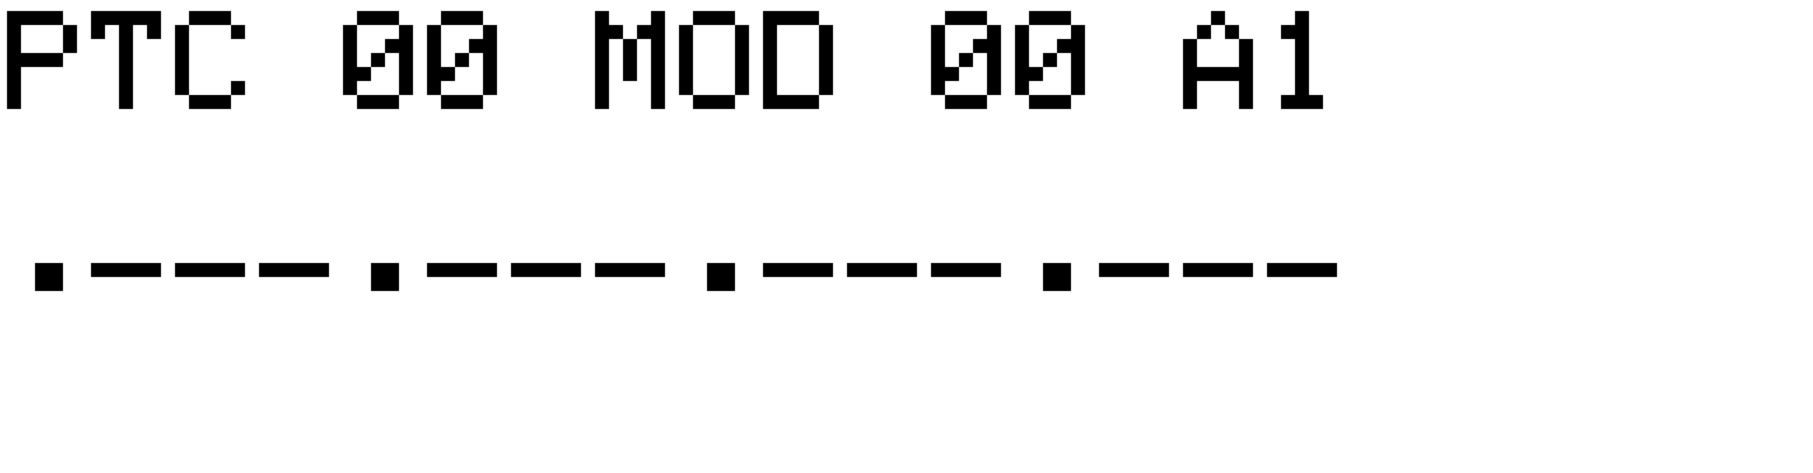
\includegraphics[scale=.40]{lockless_trigs.png}}\\
\textit{Triggers on steps 1, 5, 9 ,13. No locks.\\
Trigs can only be added or removed from the} StepEdit page.\\
\section{Locked Trigs:}
\fbox{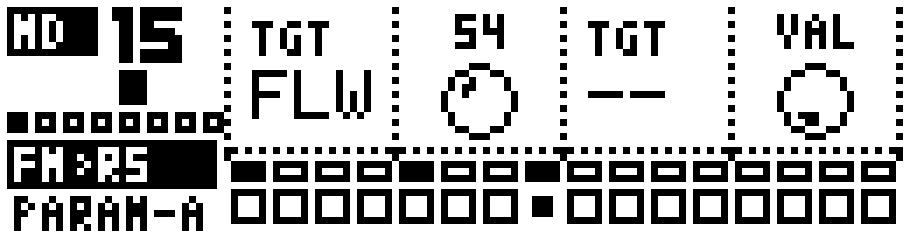
\includegraphics[scale=.40]{locked_trigs.png}}\\
\textit{Triggers and locks on steps 1, 5, 9, 13.\\}
\section{Trigless Locks:}
\fbox{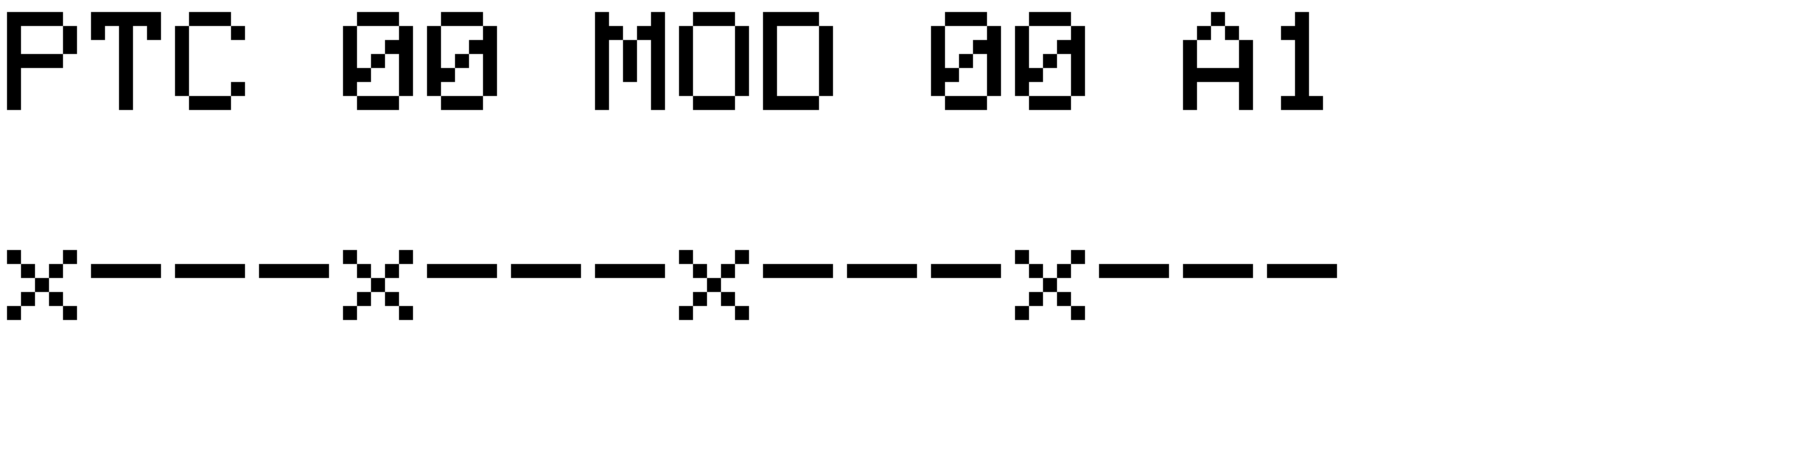
\includegraphics[scale=.40]{trigless_locks.png}}\\
\textit{Locks on steps 1,5,9,13 . No triggers}

\chapter{Parameter Lock Record  Page:}
The RLCK Page is used to record Parameter Locks in real-time. If the sequencer is running, any parameter changes on the MD will be recorded.\\
\\
\fbox{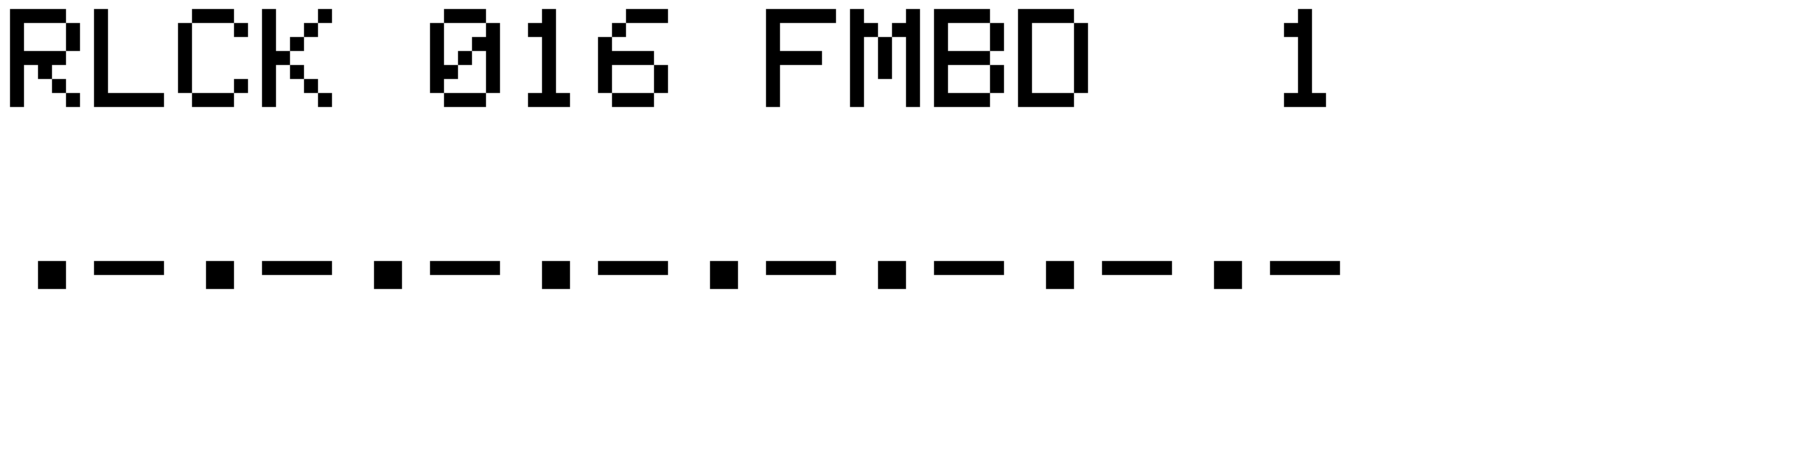
\includegraphics[scale=.40]{rlck_page_init.png}}\\
\textit{To enter the RLCK Page: Enter the RTRK Edit mode by pressing \textbf{[ Encoder 2 ]} from the Grid Page. Press the \textbf{[ Save ]} button to enter RLCK mode.}
\section{Parameter MIDI Learn}
Any MD parameter changes in the RLCK Page will be automatically learned. If a free parameter lock slot is available, it will automatically be assigned to the last Parameter received. \\
\\
When in RLCK Page, the current sequencer Track will automatically change according to the track of the last MD Parameter modified. 

\section{Encoder Assignment:}
\begin{itemize}
	\item \textbf{[ Encoder 1 ]: } --
	\item \textbf{[ Encoder 2 ]: } --
	\item \textbf{[ Encoder 3 ]: } Track Length
	\item \textbf{[ Encoder 4 ]: } --
\end{itemize}
\section{Clearing:}
\begin{itemize}
\item To clear the current track of all parameter locks, press the \textbf{[ Write ] }(top right)
\item To clear all MD tracks of all parameter locks,  press \textbf{[ Shift2 ] + [ Write ]}
\end{itemize}
\section{Rotating visible sequence:}
Each track consists of 4 pages of 16 steps, for a total of 64 steps per track.
\begin{enumerate}
	\item Rotate the current track-page by pressing the \textbf{[Shift1] }button.
\end{enumerate}
\section{Changing track length:}
\begin{enumerate}
	\item Track length is controlled by rotating \textbf{[ Encoder 3 ]}. Only steps less than the current track length are drawn.
	\item To change the lengths of all 16 tracks simultaneously hold down \textbf{[Shift 2]} whilst rotating \textbf{[ Encoder 3 ]}.
\end{enumerate}

\chapter{Parameter Edit Pages:}
The ParamEdit Pages are used to add or remove Locks to the track’s sequence.
\\

There are two dedicated pages used to edit the four Parameter locks per track.\\
Each page can be used to edit two parameters at a time.
\\

Unassigned parameters or locks are indicated by a ‘--’.

\screenshot{locked_trigs.png}
%\fbox{\includegraphics[scale=.40]{}}

\textit{To enter the ParamEdit Page:\\ Select desired track on MD by pressing \textbf{[ Function ] + [ Track n ]}. Enter the ParamEdit-A mode by pressing \textbf{[ Shift1|PageSelect ]} and \textbf{[ Trigger 5 ]}.}
\\\\
\textit{Pressing \textbf{[ Save ]} button will toggle between the available Parameter Edit Pages.}

\encodersbuttons{Param Type 1}{Step Value}{Param Type 2}{Step Value}{Toggle PARAM-A/PARAM-B}{PageSelect}{Rotate View}{Track/Trig Menu}

\section{Setting step locks:}
To change a Parameter type rotate \textbf{[ Encoder 1 ]} or \textbf{ Encoder 3 ]}.\\
To change a Parameter Value for a specific step:
\begin{itemize}
\item Press and hold one or more triggers on the MD trigger interface
\item Rotate encoders 2 or 4 to specify the parameter lock value for the specific step(s).
\end{itemize}
For each track parameter locks are automatically MIDI learnt. If a free parameter lock slot is available, it will automatically be assigned to the last Parameter received. 
\section{Clearing Locks:}
\begin{itemize}
\item To clear the current track of all parameter locks, press the \textbf{[ Load  ]}
\item To clear all MD tracks of all parameter locks, \textbf{[ Load ] + [ Shift2 ]}
\end{itemize}
\chapter{Chromatic Page:}
The PTC page, also known as the Chromatic Page, is used to play MD tracks chromatically using the MD Trigger interface or an attached MIDI Keyboard.

\screenshot{chroma.png}

For supported track types, the Track’s Pitch is mapped to Notes of a selected scale across the MD Trigger interface.

Melodies can be recorded in real-time.


%\fbox{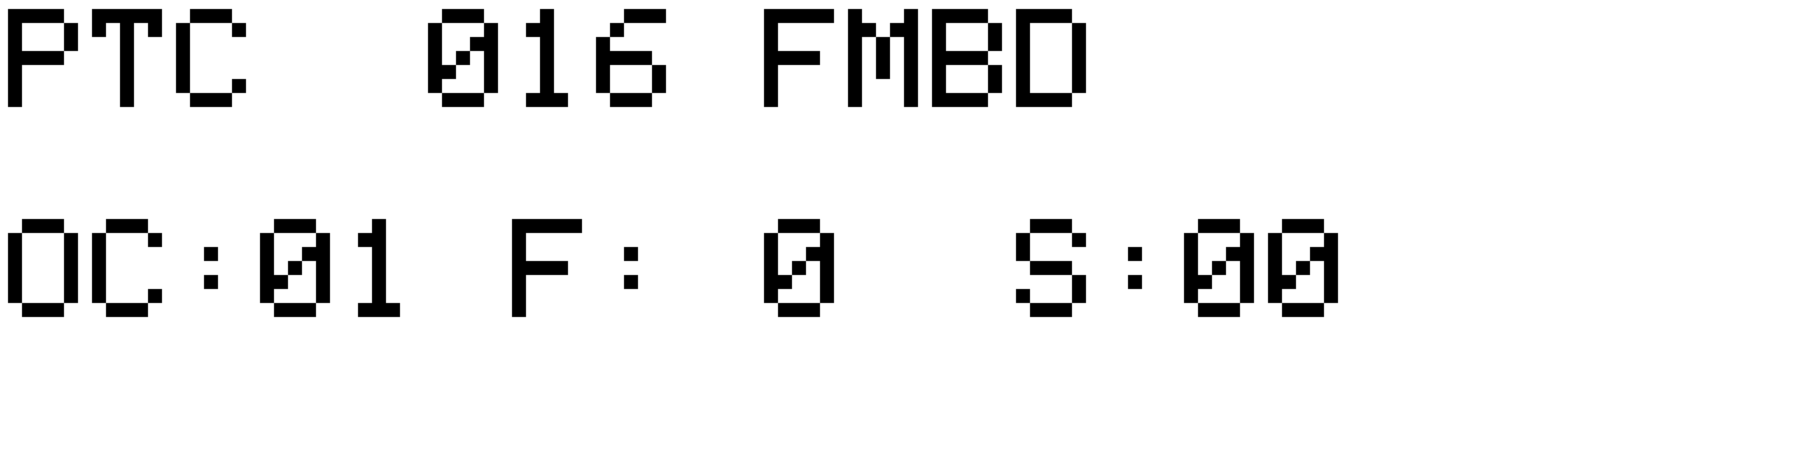
\includegraphics[scale=.40]{ptc_md.png}}\\\\



\textit{To enter the PTC Page: Select desired track on MD by pressing \textbf{[ Function ] + [ Track N ]}. Enter the PTC mode by pressing \textbf{[Shift1|PageSelect]} and \textbf{[Trigger 8] }.}

\screenshot{chromat_action.png}

\textit{A keyboard will be displayed showing the current active notes.}
\\

\encodersbuttons{Octave (OC)}{Fine Tune (F)}{Track Length}{Scale Type (S)}{Toggle PTC/RPTC}{PageSelect}{Clear Track}{Track/Trig Menu}
	
\section{A4 + ExtMIDI:}
The PTC Page is also used to record/play the Analog4 or ExtMIDI tracks. Scale modes are also supported for these track types.\\
\fbox{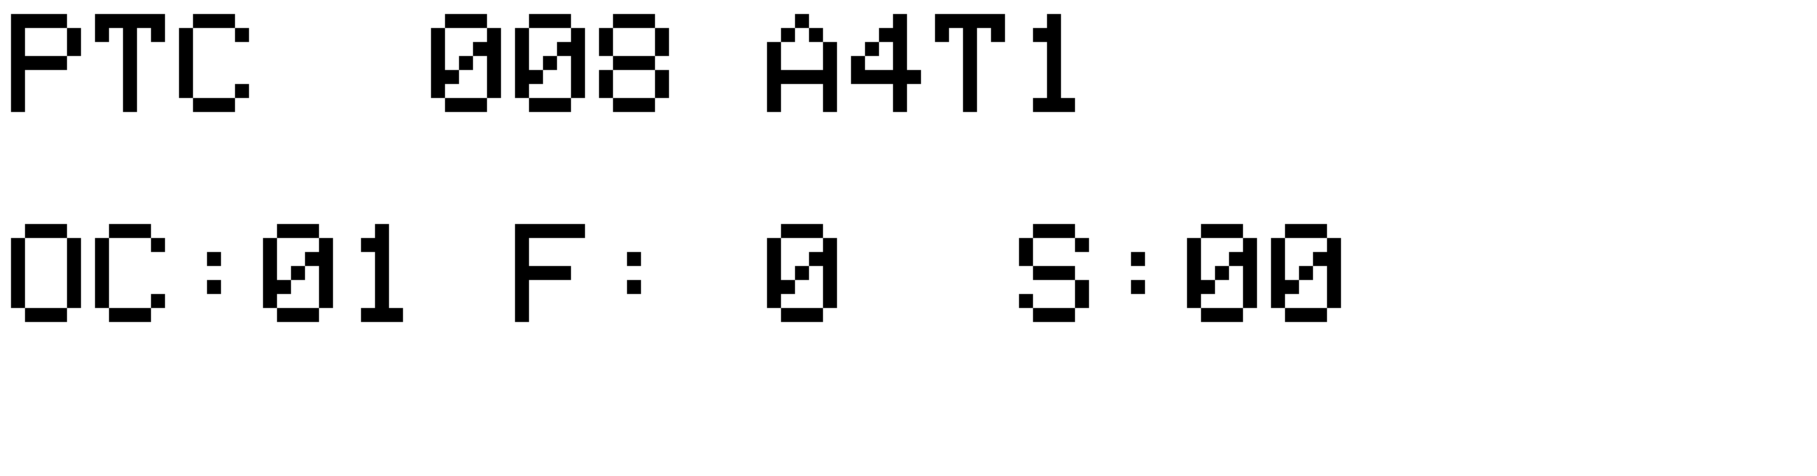
\includegraphics[scale=.40]{ptc_a4.png}}

\section{Recording a sequence:}
\textit{Press the \textbf{[ Save ] }button to enable record mode, RPTC.\\}

Play notes on either the MD or A4/ExtMidi to record a melody.

\vspace{-0.3cm}

\section{Clearing recorded sequence:}
\begin{itemize}
\item To clear the current track, press and hold the\textbf{ [ Shift2 ]} to open the track menu, rotate \textbf{[Encoder2]} to the entry \textbf{CLEAR}, then rotate \textbf{[Encoder1]} to select \textbf{TRK}.
\item To clear all tracks of the current track type, select \textbf{ALL}.
\item The current track can also be quickly cleared by pressing \textbf{[Write]}.
\end{itemize}


\vspace{-0.3cm}

\section{Changing track length:}
\begin{itemize}
\item Track length is controlled by rotating \textbf{[ Encoder 3 ]}.
\item To change the lengths of all tracks of the current track type, simultaneously hold down \textbf{[Write]} whilst rotating \textbf{[ Encoder 3 ]}.
\item Track length can also be set by holding \textbf{[Write]} and then selecting the corresponding step from the MD trigger interface. The track length is offset by the current track-page.
\end{itemize}


\section{A4 or ExtMidi}
Melodies and chords can be played and recorded from the Analog4 or ExtMIDI device in the PTC and RPTC pages.
\\

If using the Analog 4, select the desired track using the A4’s track select buttons. The first note played on the mini keyboard will cause the PolyStep edit page to switch to  the corresponding external sequencer track.
\\

\textit{The active device tab will switch over from MD to A4/MI, in the left information panel, when such midi notes are received.}
\\

Switching Between Low and High Resolution Modes on Poly Sequencer Tracks.
Press \textbf{[Shift2]} then rotate \textbf{[Encoder2]} to select the \textbf{TRACK RES.} entry.

\chapter{Polyphonic Mode}

\section{Voice Select Page}
The voice select page is used to assign MD tracks as polyphonic voices.\\\\
The TI is used to select voices\\\\
\fbox{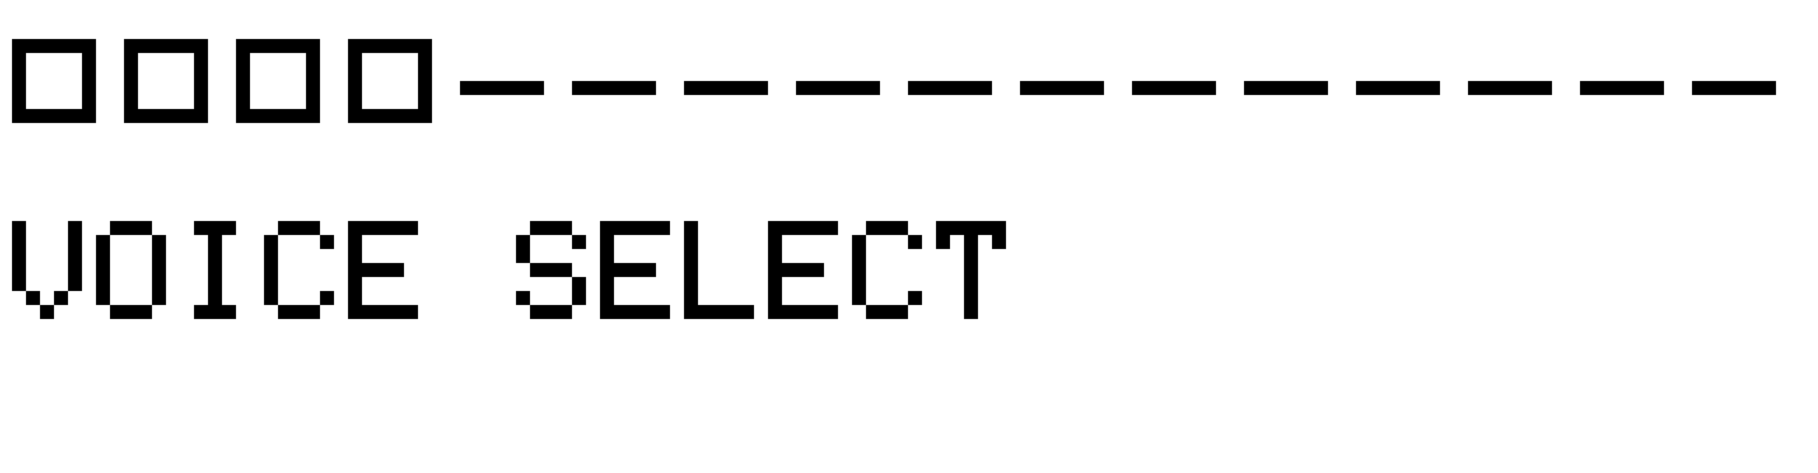
\includegraphics[scale=.40]{voice_select_page.png}}\\\\
\textit{To open the voice select page:\\\\
Enter \textbf{GlobalSettings-->MD-->POLY CONFIG}. Or press \textbf{[Save]} + \textbf{[Write]} from  Chromatic Page}

\section{Voice modes}

The Machinedrum's current active track will be used as a monophonic voice from the PTC page.\\
\\
If the current active track is part of the Polyphonic track selection \textbf{POLY} mode will be activated; the MD will be played polyphonically using voices selected from the \textbf{POLY Page.}\\
\\
When POLY mode is active, tracks become 'linked'. Track length and parameter changes will be synchronised across the voices. In addition pressing \textbf{Write} from the PTC Page will clear all recorded sequencer data from the poly tracks.

\section{External MIDI Control}
The MD can be played chromatically using an attached MIDI keyboard/sequencer connected to MIDI input port 2.
To enable/disable control from an external device you must change the Megacommand's \textbf{Global Settings->Machinedrum->CTRL CHAN} setting from INT (internal) to a desired MIDI channel or OMNI (all channels).\\
\\
When external control mode is enabled, the trigger interface will be disabled.\\
\\
You can control the voice parameters using MIDI CC messages. CC 16 to 39 control MD parameters 1 to 24 on the active track, or across all polyphonic tracks.


\chapter{Mixer Page:}
The mixer page displays the audio levels, or parameter values of the sixteen MD tracks of the current Kit.

The trigger interface is used in conjunction with \textbf{[ Encoder 1]} to raise or lower the volume of multiple tracks simultaneously. The remaining encoders can be used to adjust the filter parameters of the selected tracks. 

%\fbox{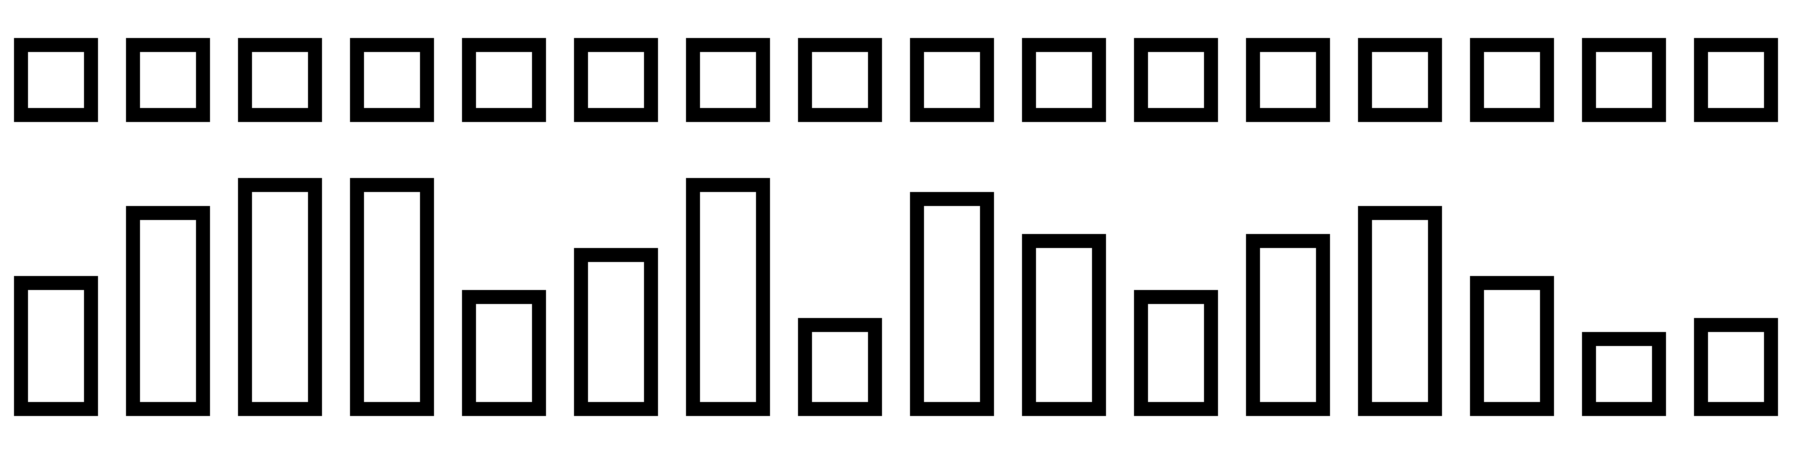
\includegraphics[scale=.40]{mixer_page_init.png}}\\\\
\screenshot{mixer_page_init.png}

\textit{The Mixer Page is accessible from the PageSelect page.}

\encoders{Level}{FLTF (Filter Frequency)}{FLTW (Filter width)}{FLTQ (Filter resonance)}

\vspace{-0.4cm}

\section{Audio Mutes}
\vspace{-0.2cm}

The top row of mixer page shows the Audio Mute state of each Track. The audio mute state changes the audio routing of muted tracks. When a track is muted from the Mixer Page, audio is routed to the Audio Output specified on the Route Page.\\
\\
\textit{Audio mutes are independent from the MD's sequencer mute page.}
\subsection{Mute Tracks}Holding down \textbf{[ Chain ]} and pressing a trigger buttons on the MD allows you to quickly toggle the mute state of a track.
\subsection{Solo Tracks}
Holding down \textbf{[ Save ]} and pressing the trigger buttons on the MD allows you to quickly solo selected tracks.
\subsection{Recall Tracks}
When entering the Mixer page, a snapshot will be taken for Level, FLTF, FLTW and FLTQ.
Holding down \textbf{[Shift2]} and pressing the trigger buttons on the MD recalls these parameter settings.

 \chapter{Route Page:}
 The (Audio) Route Page is used to send the audio of a specific MD track to a selected output. \\
 \\\textbf{[ Encoder 1]} can be used to select the audio output to MD external outputs C -> F.\\

\fbox{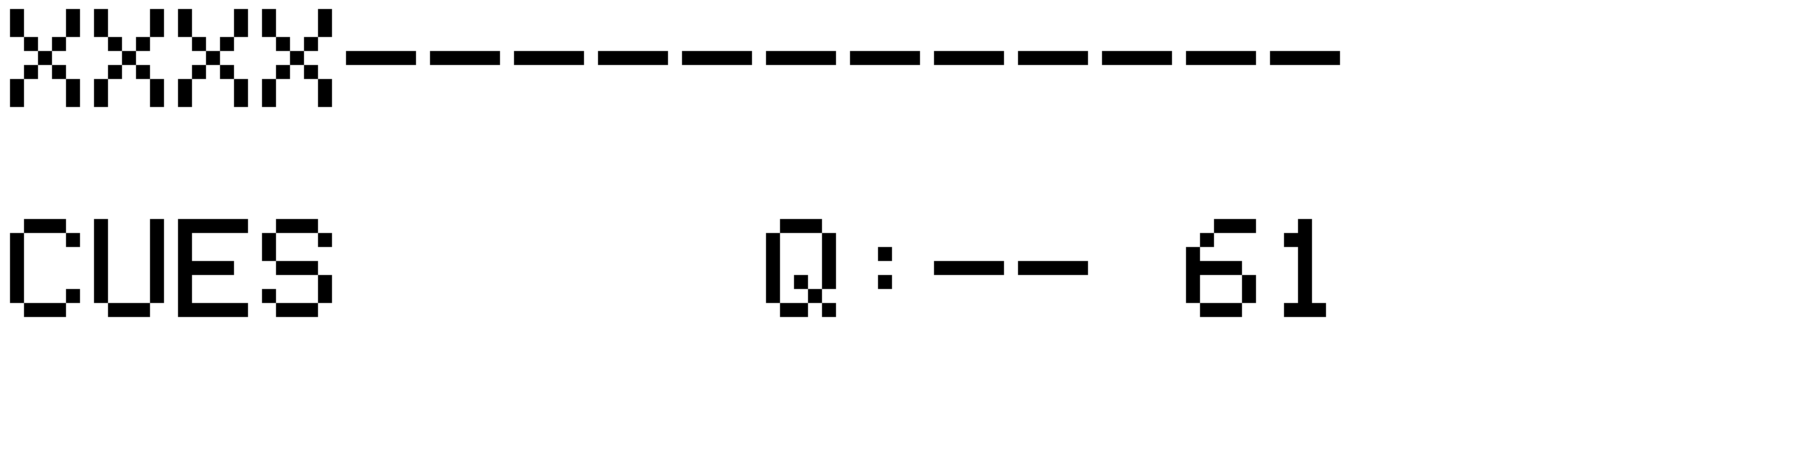
\includegraphics[scale=.40]{cue_page.png}}\\\\
 \textit{The Route Page is accessible from the PageSelect page.}
  \section{Encoder Assignment:}
 \begin{itemize}
 	\item \textbf{[ Encoder 1 ]: } Output Selection
 	\item \textbf{[ Encoder 2 ]: } --
 	\item \textbf{[ Encoder 3 ]: } Quantization
 	\item \textbf{[ Encoder 4 ]: } --
 \end{itemize}
  The trigger interface used to toggle the output of selected tracks, between Main Outputs and the chosen external output.
 \section{Quantization Modes:}
 Quantization modes are used to control the behaviour of the cue operations and allow for cue events to be musically timed.\\
 \\
 When a numerical quantization value is chosen the selected track’s cue will be toggled on the next specified multiple of the step-count.
 \begin{itemize}
\item --: No quantization.
\item 02: Toggle cue on next possible 2nd step
\item 04: Toggle cue on next possible 4th step
\item 08: Toggle cue on next possible 8th step 
\item 16: Toggle cue on next possible 16th step 
\item 32: Toggle cue on next possible 32th step 
\item 64: Toggle cue on next possible 64th step
 \end{itemize}
 
 
\chapter{LFO Page:}
The MCL firmware is equipped with its own LFO modulation source, and controls both track parameters and master FX parameters.

\screenshot{lfo.png}
\textit{To enter the LFO Page: press and hold \textbf{[ Shift1|PageSelect ]}, then press \textbf{[ Trigger 4 ]}.}

By default the LFO engine is deactivated. To toggle it ON, press \textbf{[ Save ]}.

\buttons{Toggle LFO ON/OFF}{PageSelect}{Toggle MOD/DST}{LFO Mode}

\section{Modulation Source}

The modulation source shape, speed and depth can be controlled. The subpage index will show as ``LFO>MOD'' on the left information panel.

\screenshot{lfo_action.png}

\newpage

\encoders{Waveform}{LFO Speed}{Target 1 Depth}{Target 2 Depth}

\section{Modulation Target}
To switch to the Modulation Target subpage, press \textbf{[Shift2]}. The subpage index will show as ``LFO>DST'' on the left information panel.

\screenshot{lfo_action_trig3.png}

Only valid parameter types for the current target track will be shown for Encoder2/Encoder4. Master FX machines are regarded as individual tracks, each with its own modulation target parameter types. This extends the mastering capabilities of MD, for that one can use the LFOs to create sidechain-like effects etc.

\encoders{Target Machine 1}{Param Type 1}{Target Machine 2}{Param Type 2}

\section{LFO Operation Modes}

The LFO engine operates in different modes, namely \textbf{FREE}, \textbf{TRIG}, \textbf{ONESHOT}. Use \textbf{[ Load ]} to switch between them.
\begin{itemize}
    \item FREE: Free-running LFO.
    \item TRIG: The LFO is reset on each trig.
    \item ONESHOT: The LFO is reset each trig but only plays through one cycle
\end{itemize}
\section{Parameter Offset}
The LFO modulation is relative to the destination parameter's original value (the lfo offset). The lfo offset will automatically be updated by adjusting the corresponding parameter on the MD's parameter page. For FX parameters it is best to adjust the offset from the FX Pages as changes in the MD FX page will not be immediately received by the MC.
\chapter{Sound Browser Page:}
The Sound Browser page is used to store and recall sounds from the Machinedrum.

\screenshot{sound_manager.png}
 \textit{The Sound Page is accessible from the PageSelect page.}


A sound can consist of machine settings from a single track, or two linked tracks.\\
\\
Two tracks can be linked by configuring the TrigGroup settings on one, to trigger the other. When two tracks are linked, both the source and destination track machine settings will be stored together to form a single sound.

%\fbox{
\includegraphics[scale=.40]{sound_page.png}}
\screenshot{sound_page.png}

 \section{Navigating the Sound Browser page.}
Rotate \textbf{[ Encoder 2 ]} to iterate through the menu items.\\
Press \textbf{[ Load ]} to make your selection.

The \textbf{[ Save ]} buttons can be used to exit/cancel.
 
 \section{Saving Sounds}
 To save a new Sound. 
\begin{enumerate}
 \item Select the desired track on the MD.
 \item From the Sound Page, select save.
\end{enumerate}
\section{Loading Sounds}
To load a new sound, select the sound the from the Sound Browser page.
\newpage
\section{Delete or Rename Sounds:}
\screenshot{file_menu.png}
\textit{From within the Sound Browser, press and hold \textbf{[ Shift2 ]} to access the file options menu.}\\\\
From the file options menu, you can delete or rename sound files or create new directories.\\\\\\
Use the encoder to make your selection, release \textbf{[ Shift2 ]} to activate your choice.

\chapter{Loudness Page}
Gain staging and loudness levels on the MD have always been an issue.

As a general rule of thumb, the track LEV parmater should control the absolute volume of a track where as the VOL parameter should be used to control relative level to other tracks. This means that you can confidently set a sounds level to it's maximum by turning the LEV paramater to 127, and not unexpectedly exceed it.


When working on different kits you can end up with completely different loudness levels, depending on your style of programming and the configuration of master effects.

The new firmware features a Loudness page with 3 functions that attempts to address this.

Functions:

**Track Level Normalise:** When activated,  all track levels have their LEV boosted to 127, and parameters controlling VOL (including parameter locks) are lowered to compensate. 

The resulting track loudness remains the same, but the Track LEV parameter is no longer set arbitrarily. LEV == 127 will always be the loudest volume for a track.

Gain Boost:

The ability to boost / reduce the VOL of all tracks in the current kit by a percentage amount.

Peak Analyser.

The MD is instructed to record 1 Bar of the current pattern. The recording is transferred to the MegaCommand and the WAV file is decoded and analysed. The peak value in the recording is found and this is used to determine an appropriate gain boost to increase pattern/kit loudness using the Boost function above.
\chapter{FX Delay Page}


Controls the master FX Delay settings.


\screenshot{delay.png}
\textit{The FX Delay Page is accessible from the PageSelect page.}

All the parameters of the delay effect can be controlled. Four of them are displayed at once on screen. Press the \textbf{[Save]} button to toggle between the two groups.

\section{FX A}
\encoders{Modulation(MOD)}{Modulation Frequency(MFQ)}{Mono(MON)}{Level(LEV)}
\screenshot{delay_action_2.png}

\newpage
\section{FX B}
\encoders{Delay Time(TIM)}{Delay Feedback(FB)}{Filter Frequency(FLF)}{Filter Width(FLW)}
\screenshot{delay_action.png}

\chapter{FX Reverb Page}
Controls the master FX Reverb settings.

\screenshot{reverb.png}
\textit{The FX Reverb Page is accessible from the PageSelect page.}

All the parameters of the reverb effect can be controlled. Four of them are displayed at once on screen. Press the \textbf{[Save]} button to toggle between the two groups.

\section{FX A}
\encoders{Damping(DMP)}{Gating(GAT)}{Pre-delay(PRE)}{Level(LEV)}
\screenshot{reverb_action_2.png}

\newpage
\section{FX B}
\encoders{Decay Level(DVL)}{Decay(DEC)}{Low Pass Filter(LP)}{High Pass Filter(HP)}
\screenshot{reverb_action.png}

\chapter{RAM Page:}
A RAM page is used to automate the recording and playback of the MD's RAM machines. The MCL firmware is equipped with two RAM Pages.
\\\\
A RAM page can be used to sample the MD main outputs or the External Inputs in either Mono or Stereo. The recorded loop can then be played.
Slicing with the various 'slice modes' allows for interesting musical and performance effects.
\\\\
RAM Page 1 will record and playback on MD track 15\\
RAM Page 2 will record and playback on MD track 16\\
\\
\textit{When stereo mode is enabled from Global Settings->Aux Pages->RAMPage, the recording and playback of RAM machines on track 15 + 16 are linked.}
\screenshot{ram1.png}
\\
\textit{To enter RAM Page one or two: \\Press and hold
\textbf{[ Shift1|PageSelect ]}, then press \textbf{[ Trigger 15 ]} or \textbf{[ Trigger 16 ]}.}
\screenshot{ram1_action.png}

\encoders{Record Source}{Slice Modulation}{Number of Slices}{Record/Playback Length}
\buttons{Record}{PageSelect}{Play}{Slice Mode Toggle}
\newpage
\section{Recording:}
\begin{itemize}
    \item{To use the RAM Machines, first start playing a pattern on the MD.}
    \item{Leave tracks 15 + 16 available as these will be overwritten for RAM machine sampling and playback.}
    \item{From the RAM Page, choose the recording source. INT for sampling the MD internal sound engine. Select the recording length and press \textbf{[ Save ]} to initiate recording. Recording is quantized with respect to the chosen length.}
    \item The status text "Queue" will be displayed indicating that record event is about to occur. The status text "Recording" will be displayed indicating that the RAM machines are recording. Recording is continuous and can only be stopped by initiating playback.
\end{itemize}

\section{Playback:}
\begin{itemize}
\item Press \textbf{[ Load ]} to initiate playback. The status text "Queue" will be displayed indicating that play event is about to occur. 
\item The status text "Playback" will be displayed indicating that the RAM machine(s) are playing. Playback is continuous until recording is re-initiated. 
\end{itemize}


\section{Mono:}
When in Mono mode RAM machines can either sample a mono MIX of the MD output, or external inputs A or B
\section{Stereo:}
When in Stereo mode RAM machine one will record MD output A and RAM machine 2 will record MD output B. Similarly if the recording source is set to EXT RAM machine one will record EXT input A and RAM machine 2 will record EXT input B

On playback stereo tracks are panned and linked. Parameter changes across tracks 15 and 16 are synchronised.
\newpage
\section{Slicing}
Slicing will divide the recorded sample in to N slices, and set up a playback trigger for each slice. It does this by setting start/end parameters locks for each trig/slice. The default number of slices is 1.\\
\\
To slice the recorded sample, select the number of slices using Encoder 3 and then press \textbf{[ Load ]}.
\\

\section{Slicing Modes}

The modulation modes affect how slices are played back.
\begin{itemize}
    \item 0: Reverse slices
    \item 1-4: Reverse every nth slice
    \item 5: Play slices in backwards order
    \item 6: Play slices in random order
\end{itemize}




\chapter{WAV Designer}
WAV designer is a single-cycle waveform generator optimized for the Elektron MD.\\
It features a 3 oscillator additive synthesis engine with a level mixer.\\
\\
Each oscillator can be set to a unique waveform and pitch. The 3 oscillators are then mixed together and rendered in to a WAV file which can be transferred to the MD using the MIDI Sample Dump Specification (SDS).\\
\\
To ensure that the MD plays back the resulting waveform optimally, WAV Designer performs all the heavy lifting for you. This involves calculating sample length and rate based on the fundamental frequency, auto detecting loop points and normalizing the waveform.
\section{WAV Designer Pages}
\textit{WAV Designer is accessible from the \textbf{PageSelect} page and consists of 4 sub-pages. Once you have entered the WAV Designer you can access the sub-pages using the four Encoder buttons.}

\begin{itemize}
\item \textbf{Encoders[1-3]}: select Oscillator Pages 1-3 respectively.
\item \textbf{Encoder[4]}: is the Mixer Page.
\end{itemize}

\section{Oscillator Pages:}
\subsection{Encoder Assignment:}
\begin{itemize}
	\item \textbf{[ Encoder 1 ]: } Pitch, note increments.
	\item \textbf{[ Encoder 2 ]: } Fine Tune, +/- 100 cents
	\item \textbf{[ Encoder 3 ]: } Pulse Width
	\item \textbf{[ Encoder 4 ]: } Modify
\end{itemize}
\subsection{Pitch:}
Each oscillator can run at a unique frequency.\\
\\The pitch is adjusted in note increments by rotating \textbf{[ Encoder 1 ]}. Rotating \textbf{[ Encoder 2 ]} will adjust the frequency in cents +/-100. Holding down \textbf{[ Shift 2 ]} will display the corresponding frequency.\\
\\The fundamental frequency of the rendered waveform is automatically selected from the oscillator that has the lowest frequency.
\subsection{Waveforms:}
Each oscillator can be set to a unique waveform by pressing the \textbf{[Save]} button from it's respective page.\\
\\
The available waveforms are described below:

\begin{itemize}
\item{\textbf{SIN:}}Sine waveform with adjustable overtones (each overtone is an octave above the fundamental frequency)\\
\fbox{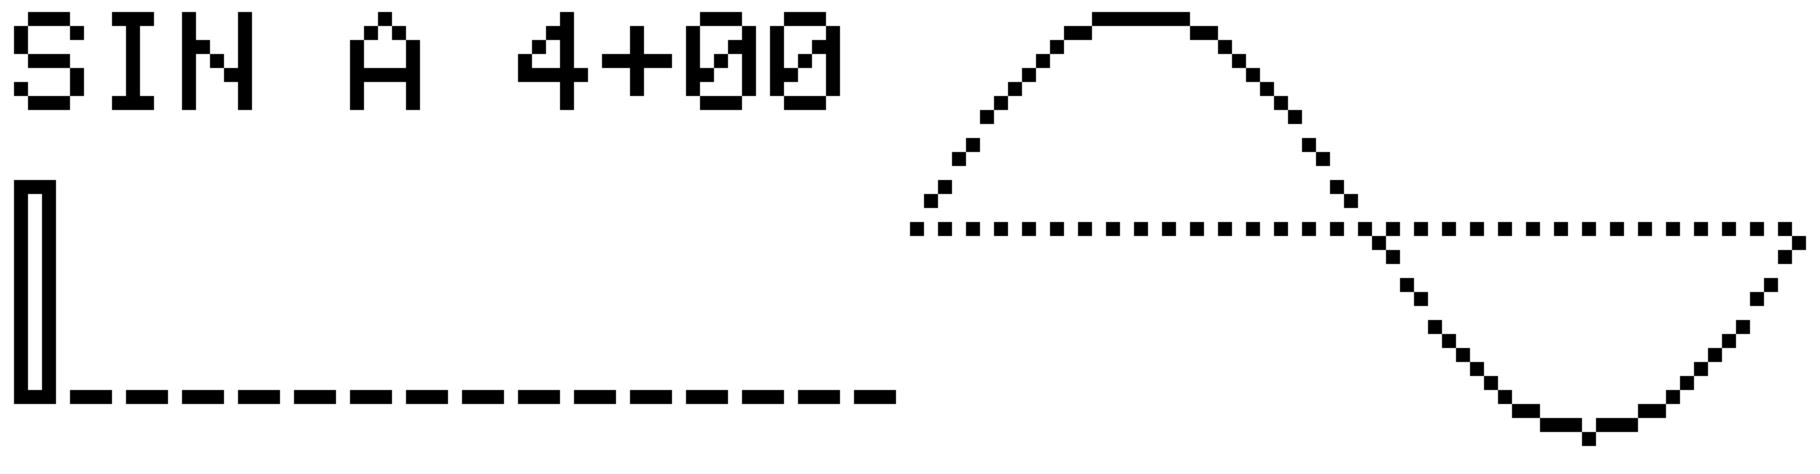
\includegraphics[scale=.40]{wav_designer_sine_init.png}}\\\\
\fbox{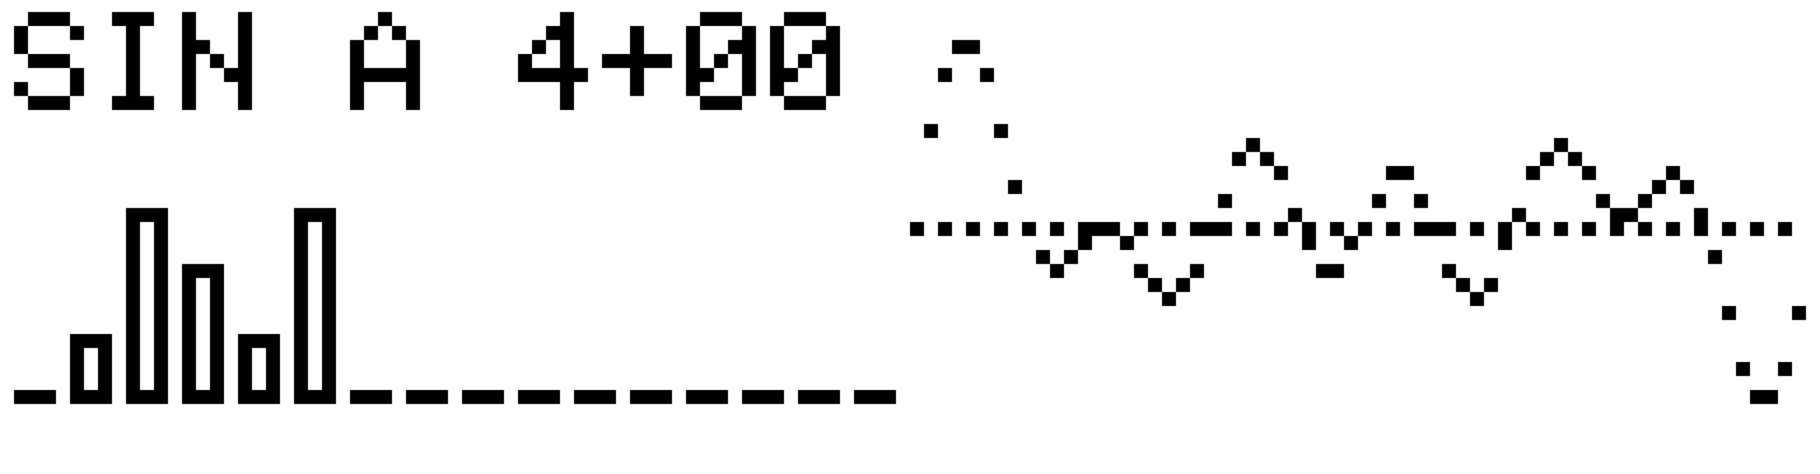
\includegraphics[scale=.40]{wav_designer_sin.png}}\\\\
\\Overtones are added by using the MD TI and rotating \textbf{[Encoder 4]}.
\item{\textbf{TRI:}} Triangle waveform with adjustable width.\\
\fbox{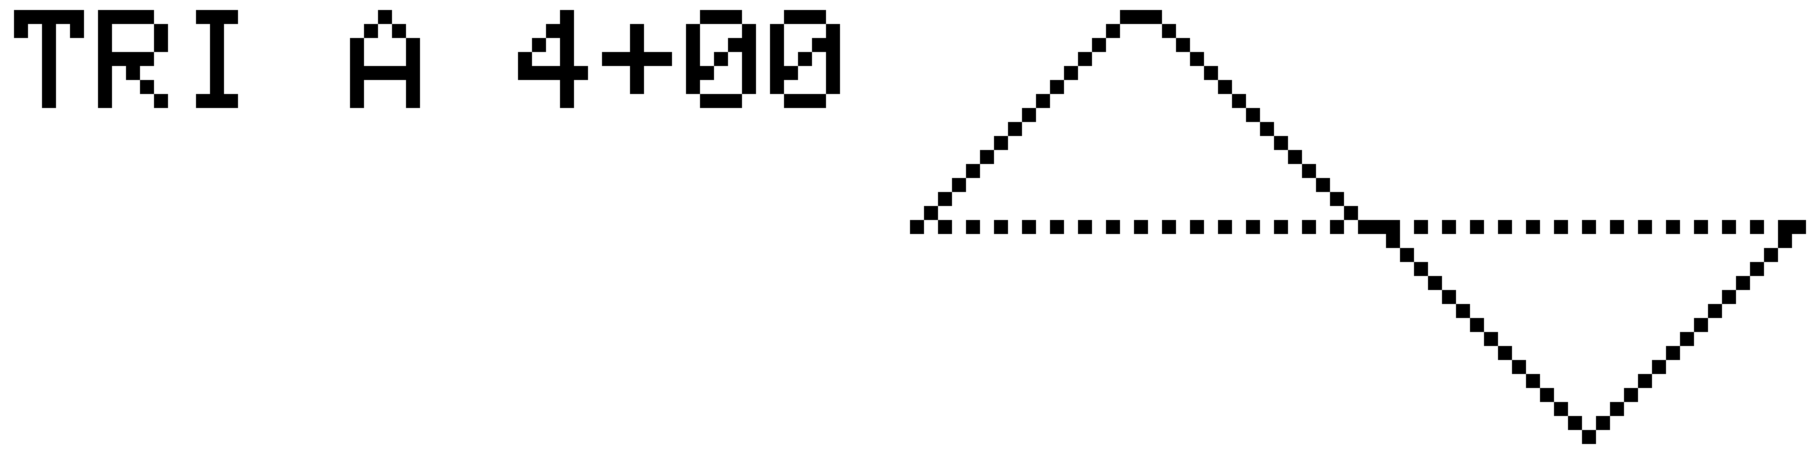
\includegraphics[scale=.40]{wav_designer_tri.png}}\\\\
\item{\textbf{PUL:}} Pulse/Square waveform with adjustable width.\\
\fbox{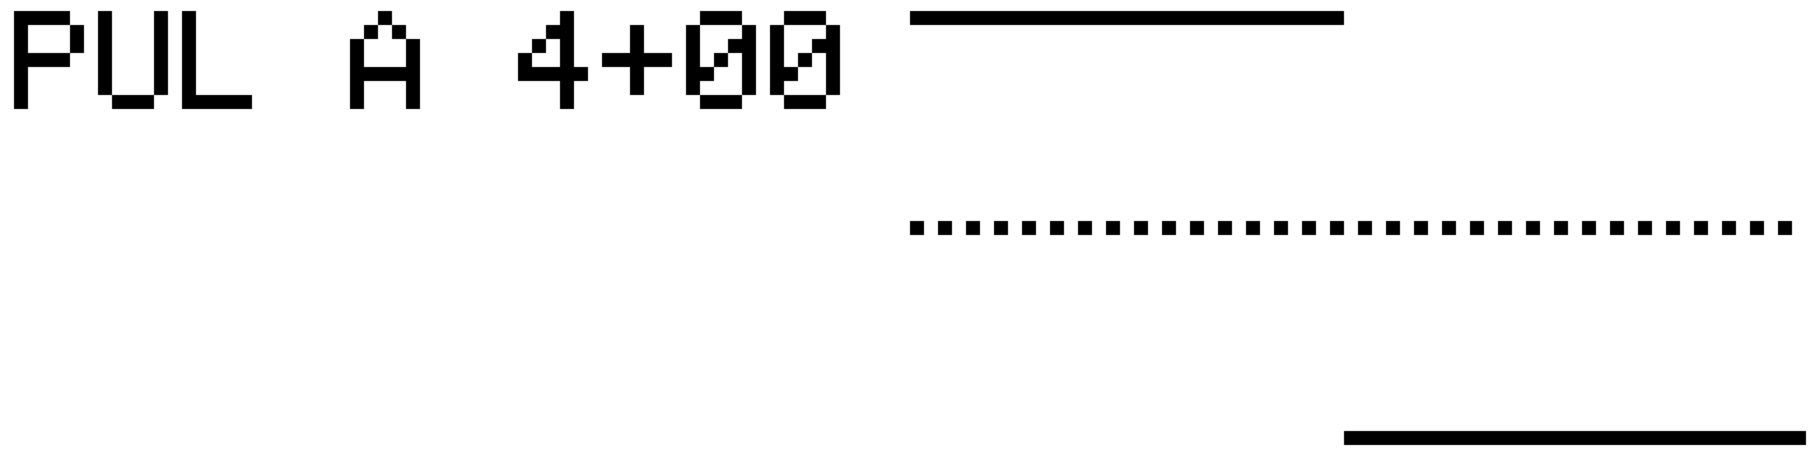
\includegraphics[scale=.40]{wav_designer_pulse.png}}\\\\
\item{\textbf{SAW:}}Sawthooth waveform with adjustable width\\
\fbox{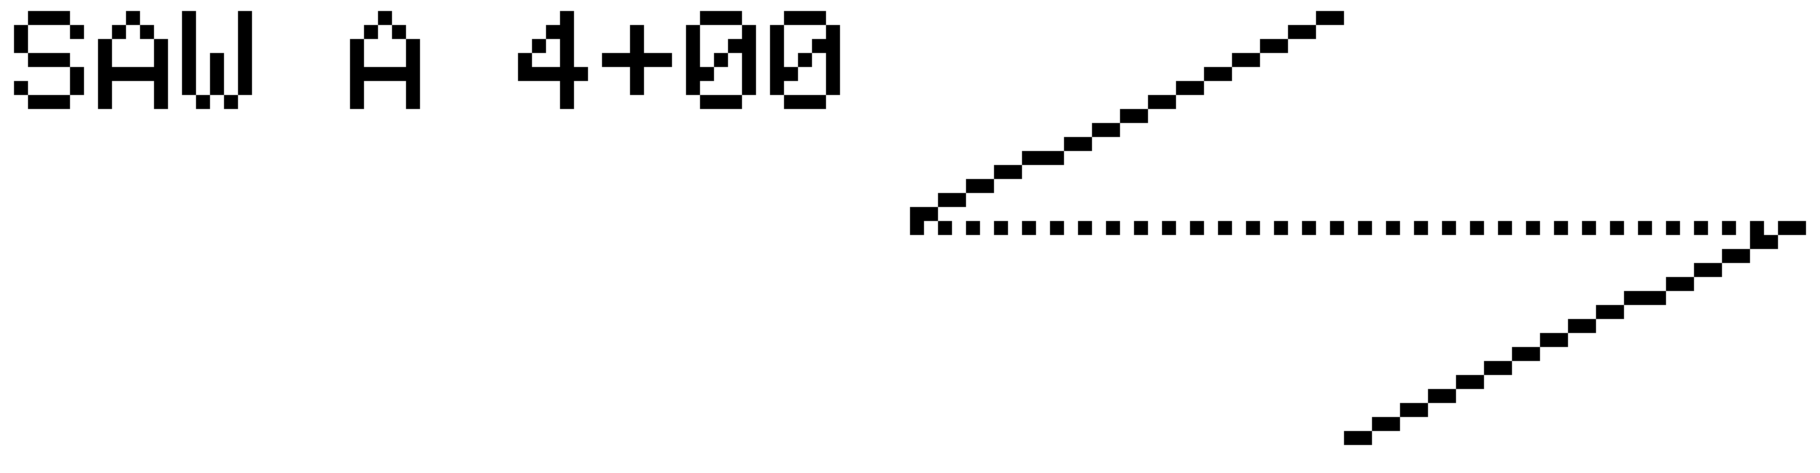
\includegraphics[scale=.40]{wav_designer_saw.png}}\\\\
\item{\textbf{USR:}}User defined waveform, 16 points with linear interpolation.\\
\fbox{
\includegraphics[scale=.40]{wav_designer_user.png}}\\\\
Sample values are modified by using the MD TI and rotating \textbf{[Encoder 4]}.
\end{itemize}
\subsection{Pulse Width:}
TRI, PULSE and SAW waveform's pulse width adjusted by rotating \textbf{[Encoder 3]}.\\
\fbox{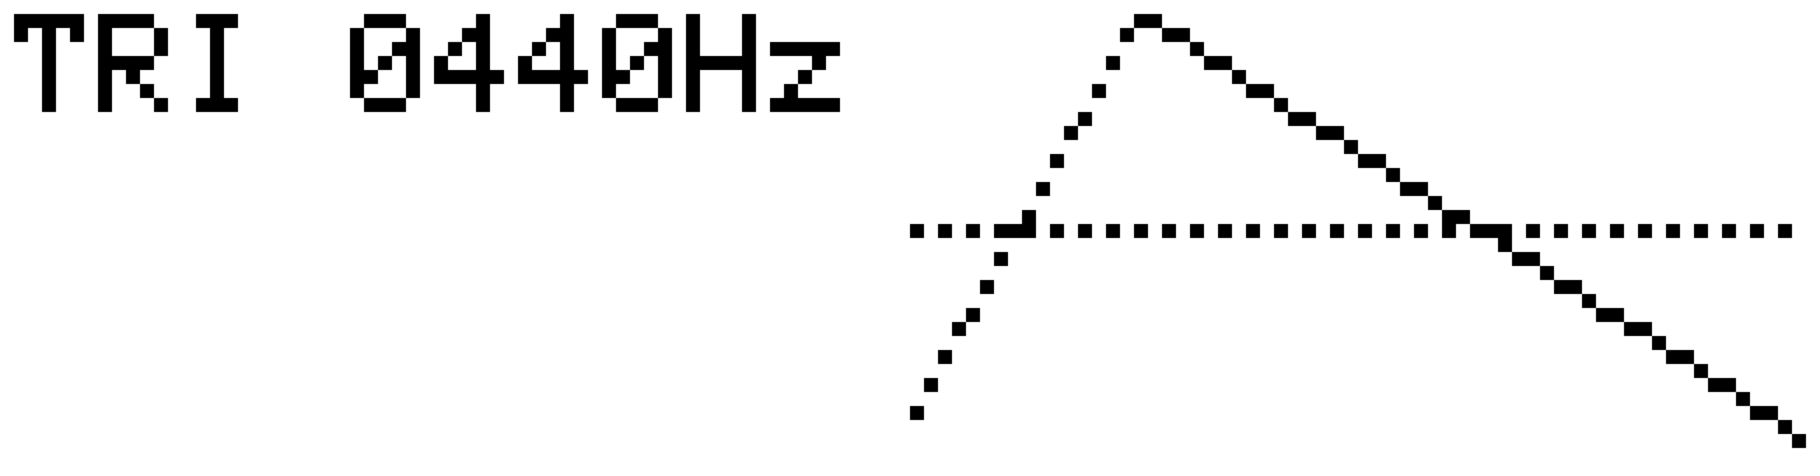
\includegraphics[scale=.40]{wav_designer_pulse_width.png}}\\
\section{Mixer Page:}
\fbox{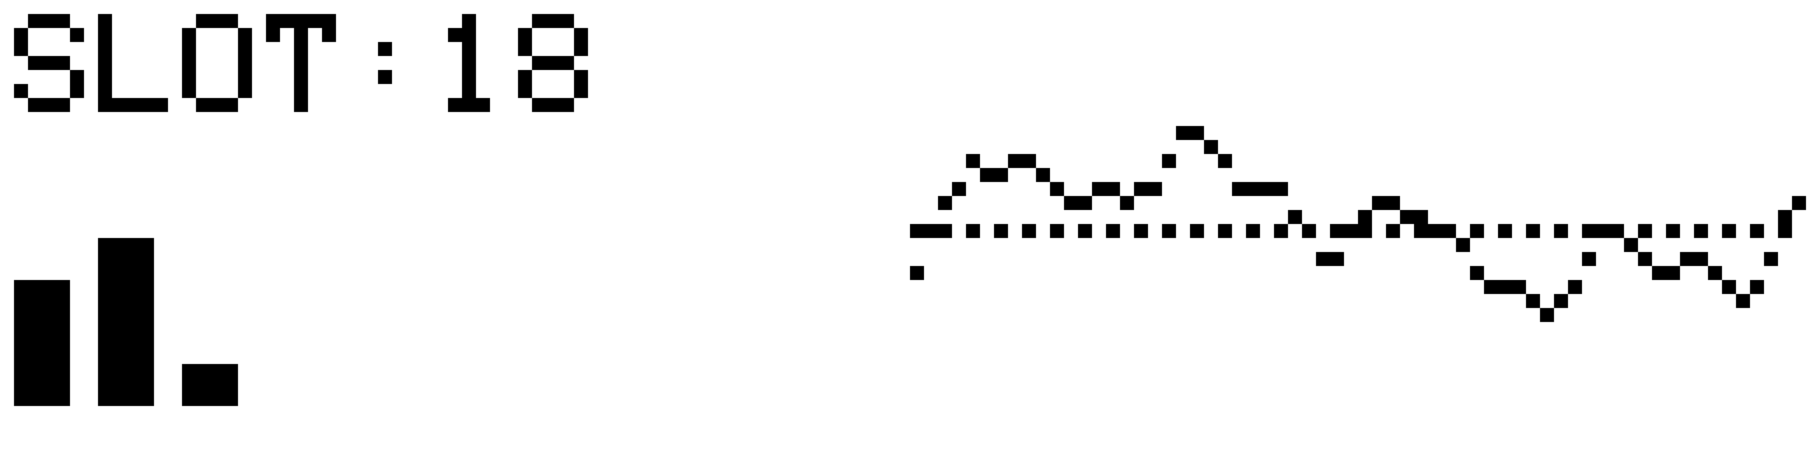
\includegraphics[scale=.40]{wav_designer_mixer.png}}\\\\
The WAV Designer mixer page has volume levels for each of the oscillators which can be adjusted by rotating encoders 1 to 3. \textit{Absolute volume levels are not important here as the resulting waveform will be automatically normalized.}

\\The fourth encoder is used to set the sample slot position. On the MD the sample slots are offset by 1 (00 = 01).\\
\\
To render a sample and then transfer it to the MD's selected sample slot, press \textbf{[Write]}.\\
\\
For convience, pressing the \textbf{[Save]} button will open the SampleManager window on the MD. You can also choose the destination slot from here.
\subsubsection{Encoder Assignment:}
\begin{itemize}
	\item \textbf{[ Encoder 1 ]: } Osc1 Level
	\item \textbf{[ Encoder 2 ]: } Osc2 Level
	\item \textbf{[ Encoder 3 ]: } Osc3 Level
	\item \textbf{[ Encoder 4 ]: } Sample Slot
\end{itemize}
\textbf{Important}: The MD firmware features a nasty bug that causes the user interface to stop responding if a sample dump is received at any point after specific SYSEX messages are requested. As MCL uses SYSEX for all communication with the MD, the MD's GUI will lock up after a sample is received from WavDesigner. The only known work around at this time is to reset the MD.
\backmatter

% bibliography, glossary and index would go here.

\end{document}